\documentclass[fontsize=11pt]{scrreprt}
\usepackage[stable]{footmisc}
\usepackage{xr}
\usepackage[utf8]{inputenc}
\usepackage{booktabs}
\usepackage{adjustbox}
\usepackage{siunitx}
\usepackage{makecell}
\usepackage[english]{babel}
\usepackage{rotating}
\usepackage{tikzpagenodes}
\usepackage[locale=DE]{siunitx}
\usepackage[section]{placeins}  % Prevents figures from floating above section headers
\sisetup{math-rm = true}
\usepackage{amssymb}
\usepackage{amsmath}
\usepackage{amsmath}
\usepackage{graphicx}
\usepackage{xcolor}  
\usepackage{pdflscape}
\usepackage[nohyperlinks]{acronym}
\graphicspath{ {images/} }
\usepackage{times}
\usepackage{color}
\usepackage{geometry}
\usepackage{setspace}
\usepackage[T1]{fontenc}

\newcommand{\hsp}{\hspace{20pt}}
\usepackage{tocloft}
\usepackage{datetime}
\usepackage{tabu}
\usepackage{fancyhdr}
\geometry{a4paper}
\usepackage[backend=biber]{biblatex}

\definecolor{jluhellblau}{RGB}{220, 230, 235}
\definecolor{pantoneblack}{RGB}{0,0,0}
\definecolor{jlugrau}{RGB}{83, 96, 107}
\definecolor{jlublau}{RGB}{0, 105, 179}
\definecolor{chaptergrey}{rgb}{0.7,0.7,0.7}
\definecolor{thmgreen}{RGB}{128,186,36}
\definecolor{thmgrau}{RGB}{74,92,102}
\definecolor{thmblau}{RGB}{0,59,209}
\definecolor{thmbhellblau}{RGB}{64,255,237}
\definecolor{ptraorange}{RGB}{240, 201, 31}

\newcommand{\thesistitle}{Bachelorarbeit} % Title of the Thesis, change here
\author{Lorenz Saalmann}
\newdateformat{monthyeardate}{%
  \monthname[\THEMONTH], \THEYEAR}

% For Figures and Subfigures
\usepackage{graphicx, caption, subcaption}
\usepackage{physics}

% Package to keep images in place
\usepackage{float}

% Package for enumerate
\usepackage{enumitem}


\addbibresource{reference.bib}

\setcapindent{0pt}

% Page Style
\pagestyle{fancy}
% Kopfzeile definieren
\fancyhead[L]{\leftmark} % Links: Kapitelname
\fancyhead[R]{\thepage}  % Rechts: Seitenzahl
\fancyfoot{}

% Line Spacing
\usepackage{setspace}

% To make uppercase words
\usepackage{textcase}

% Kapitelnummer mit Punkt formatieren
\renewcommand{\chapterformat}{\setkomafont{chapter}\chapterfont\bfseries\Huge \textcolor{gray}{\thechapter \enskip \Big|} \enskip}

\usepackage[bookmarks, colorlinks=false, pdfborder={0 0 0}, pdftitle={\thesistitle}, pdfkeywords={}]{hyperref}
\setlength{\parindent}{0pt}
\setlength{\parskip}{1em}

\begin{document}

% To expand the word spacing
\spaceskip=1.2\fontdimen2\font plus 1.2\fontdimen3\font
minus 1.2\fontdimen4\font

\begin{titlepage}
\begin{tikzpicture}[remember picture,overlay,shift={(current page.south)}]


\node [text width=13cm] at (0, 9.5)
{
\sffamily
\begin{flushleft}
    \vspace{.5cm}
    \LARGE
\color{black}
\textbf{Investigating the Effects of 
Atmospheric Pressure Plasma Radiation 
on the Sterilization of Cladosporium sphaerospermum}\\[3ex]
\vspace{.5cm}

\vspace{1cm}

\text{Lorenz Saalmann}\\[1ex]
\small\text{SS 25}\\[.9ex]
\end{flushleft}
};

\centering
\node [text width=8cm] at (0,18){
\includegraphics[width = 1\textwidth]{Logo_KIT.png}};


\node at (0,25) {
\includegraphics[width = 0.32\textwidth]{JLU.jpg}};

\end{tikzpicture}
\end{titlepage}


\setcounter{page}{1}
%% Titlepage
%  Note: all text inside < ... > has to be adapted!
{% enclose this page so what is defined here does not spill over elsewhere
\pagestyle{empty}
\setstretch{1.5}
\sffamily
%\hfill\includegraphics{logo_univie_bw}

% the switch form will also prevent hyphenation which would be undesired for a title
\vspace{1cm}
\vfill
{\bfseries \Large Spezialisierungsmodul}

{\Large as part of an internship at Kyoto Institute of Technology (KIT)}

\vspace{1cm}

{\Large Development and Ion-Optical Simulation of an
Electron-Impact Ionization Time-of-Flight Mass
Spectrometer}
\vfill

handed in by

{\Large Lorenz Saalmann}\\[1.0ex]
{\large {8104072}}\\[.2ex]
{karl.lorenz.saalmann@physik.uni-giessen.de}\\[2ex]
{\large {Student of Physics and Technology for Space Applications}}\\[.5ex]


{\large {JLU:    Dr. Kristof Holste}}\\[.5ex]
{\large {KIT:    associate Prof. Kazou Takahashi}}\\[.5ex]


\vfill



{\large {\today}}\\[.5ex]

{\large {I. Physikalisches Institut}}\\[.5ex]
{\large {Justus-Liebig-Universität Gießen}}\\[.5ex]
{\large {Gießen, Germany}}\\[.5ex]

\cleardoublepage
% \end{titlepage}
}%end of title page 

\chapter*{Abstract}
Using atmospheric pressure plasma for surface sterilization has been shown to be a promising alternative to conventional chemical and thermal methods. While the focus of most studies has been on the inactivation of bacteria, this work explores the interaction of atmospheric pressure air plasma with a fungus, Cladosporium sphaerospermum, a mould known for to be resilient. The aim of the study is to investigate the role of radiation emitted by the plasma in the sterilization process and to get a better understanding of the mechanisms that lead to inactivation.

To achieve this, three approaches are taken: optical emission spectroscopy (OES) analysis of the plasma, ultraviolet (UV) exposure experiments using a UV lamp, and plasma treatment with its radiation isolated through a quartz glass barrier. The OES results identified the Second Positive System (2PS) of molecular nitrogen as the main source of UV emission. The wavelengths emitted are primarily between 300 nm and 400 nm. An approximate electron temperature of 6500 K was calculated using a Boltzmann plot. The exposure experiments showed that a UV dose of 0.35 mJ/cm² effectively inactivated C. sphaerospermum spores, while the plasma treatment with the quartz barrier achieved a 50\% inactivation rate after 30 minutes. This proves that the radiation emitted by the APP significantly contributes to the sterilization process. However, the effects of the hydroxyl radicals could not be fully isolated with the setup, the results suggest that the radiation plays a significant role in the inactivation of spores, but further research is needed to quantify its contribution accurately.
\cleardoublepage

\tableofcontents
\cleardoublepage

\listoffigures
\listoftables
\section*{\huge List of Abbreviations}
\begin{acronym}
  \acro{eu}[2PS]{\dotfill Second Positive System}
  \acro{eu}[APP]{\dotfill Atmospheric Pressure Plasma}
  \acro{eu}[C. Sphaerospermum]{\dotfill Cladosporium Sphaerospermum}
  \acro{eu}[DBD]{\dotfill Dielectric Barrier Discharge}
  \acro{eu}[EEDF]{\dotfill Electron Energy Distribution Function}
  \acro{eu}[ISS]{\dotfill International Space Station}
  \acro{eu}[KIT]{\dotfill Kyoto Institute of Technology}
  \acro{eu}[OES]{\dotfill Optical Emission Spectroscopy}
  \acro{eu}[UV]{\dotfill Ultraviolet}

\end{acronym}
\cleardoublepage

% Main Content
\onehalfspacing

\cleardoublepage

\chapter{Introduction}
\label{chap:intro}
In various industries, including medical, agricultural fields and aerospace fields, the sterilization of surfaces or equipment is an ongoing challenge that still shows room for improvement. Many sterilization methods rely on the use of chemicals or high temperatures around 120 \textdegree C. This can be problematic as it can damage or fatigue materials and leave traces of toxic gases like formaldehyde \cite{app_study}. Using a plasma instead of chemicals or heat has been shown to be a promising alternative. Especially the use of atmospheric pressure plasmas (APP) is a great general-purpose sterilization method, as the plasma can be generated without the need for a vacuum chamber. APPs are generally non-thermal, can be created around room temperature and don't need to be in direct contact with the materials they interact with. This allows for the treatment of sensitive materials and fine adjustment of the intensity by varying distance and time of exposure. 

In the past the treatment of bacteria with APPs has been the focus of many studies \cite{app_study,bacteria}, however another group of microorganisms, fungi, which include moulds, has not been studied as much. Moulds are known to be more resistant to sterilization than bacteria and are ubiquitous in virtually all environments. Many of the conventional methods fall short of effectively eradicating the spores of moulds especially in porous surfaces. This is a problem in the food industry, where moulds can spoil food and cause allergic reactions in humans but also in households \cite{mould, growth}.

It is known that the sterilization effect that APPs have on microorganisms is related primarily to reactive species that are formed in the plasma. Studies have also proposed that the radiation emitted by the plasma contributes to this, but it is not clear how much of the effect can be attributed to the radiation. The aim of this work is to investigate the effect of APPs on the mould Cladosporium sphaerospermum and to dissect the role of the radiation, specifically in the ultraviolet (UV) range, in the sterilization process. To research this the study tries to answer the following three questions:
\begin{itemize}
    \item Can UV radiation effectively inactivate spores of Cladosporium sphaerospermum?
    \item Does the APP used in this experiment emit UV at wavelengths known to be effective in spore inactivation?
    \item Does plasma-emitted radiation alone produce a sterilization effect on Cladosporium sphaerospermum spores, and how much of the overall effect can be attributed to this radiation?
\end{itemize}

To investigate these questions multiple experiments are designed and conducted during a 4-week internship at the Kyoto Institute of Technology (KIT) in Japan. At first, the plasma and the spores are separated in two experiments. One measures the inactivation of spores by UV radiation and the other analyses the optical spectrum of the plasma. Then the spores are treated with the APP and the effect of the radiation is isolated by using a transparent quartz glass barrier between the plasma and the spores. The results are then compared to the inactivation without the barrier to determine the effect of the radiation. Finally, they are analysed and discussed in the context of prior studies.

Because the mould needs multiple days of incubation time, more literature research was done in parallel. The next chapter provides scientific context on the use of plasmas for sterilization, followed by some theory on the mould Cladosporium sphaerospermum and a direct connection to the author's university research on space applications.
\chapter{Scientific Context}
\label{chap:scientific_context}
There have been many recent studies on the use of plasmas for sterilization and its effects on microorganisms \cite{bacteria, app_study, kit, wound,inactivation}. This chapter aims to provide an overview of the scientific context surrounding this topic as well as research on the interaction of fungi with radiation.

The use of plasma treatment in the medical field goes back to the 20th century. Its history is outlined well in \cite{history}. While the first plasma treatments were used on skin their antimicrobial\footnote{Inhibits the growth of microorganisms.} properties were soon discovered. In the 1990s Mounir Laroussi demonstrated the use of DBD plasma for sterilization of surfaces \cite{laroussi}. Its first use focussed on the sterilization of medical instruments and equipment where removing bacteria and viruses is crucial. With this began many studies on the interaction of plasma with bacteria, and it has been shown that DBD plasma can very effectively be used for sterilization \cite{inactivation, app_study}. With this many devices have been developed that are now used commonly in hospitals and laboratories \cite{history}. Although sterilization has been studied extensively most of the studies have focussed on the deactivation of bacteria exclusively. Recent studies have started to investigate the interaction of plasma with fungi which is relevant for the food industry and the cleaning of environments  \cite{growth}. While its efficacy has been proven well, it is not yet fully understood which processes carry responsibility for the inactivation of microorganisms especially on fungi. It is believed that the main mechanism of inactivation is the generation of reactive species in the plasma which can defuse into the cell and damage DNA and proteins \cite{app_study, inactivation}. A clear relationship between treatment time, proximity and inactivation rate has been shown. According to prior studies moulds like C. sphaerospermum are a lot more resistant to UV radiation than bacteria \cite{app_study}. 

Non-thermal plasma can however also radiate ultraviolet (UV) light and the electric field applied through DBD can also have an effect on the microorganisms. A recent study by Li, Yiqian and others \cite{bacteria} has researched the effects of the physical energy of the plasma on bacteria by separating samples with different materials transparent to radiation and electric fields and found them to have a significant effect. In this work a similar approach is taken to investigate the effects of the radiation on the fungus C. sphaerospermum. The basis for which was formed by previous work by the department for plasma physics at the Kyoto Institute of Technology done by Tomoya Ohara and others \cite{kit} where this study continued. They showed that treatment times of 20 minutes are sufficient to inactivate the fungus by more than 99 \% and measure the concentration of ozone and hydroxide ions. Figure \ref{fig:kit} shows the results of their study.

\begin{figure}
    \centering
    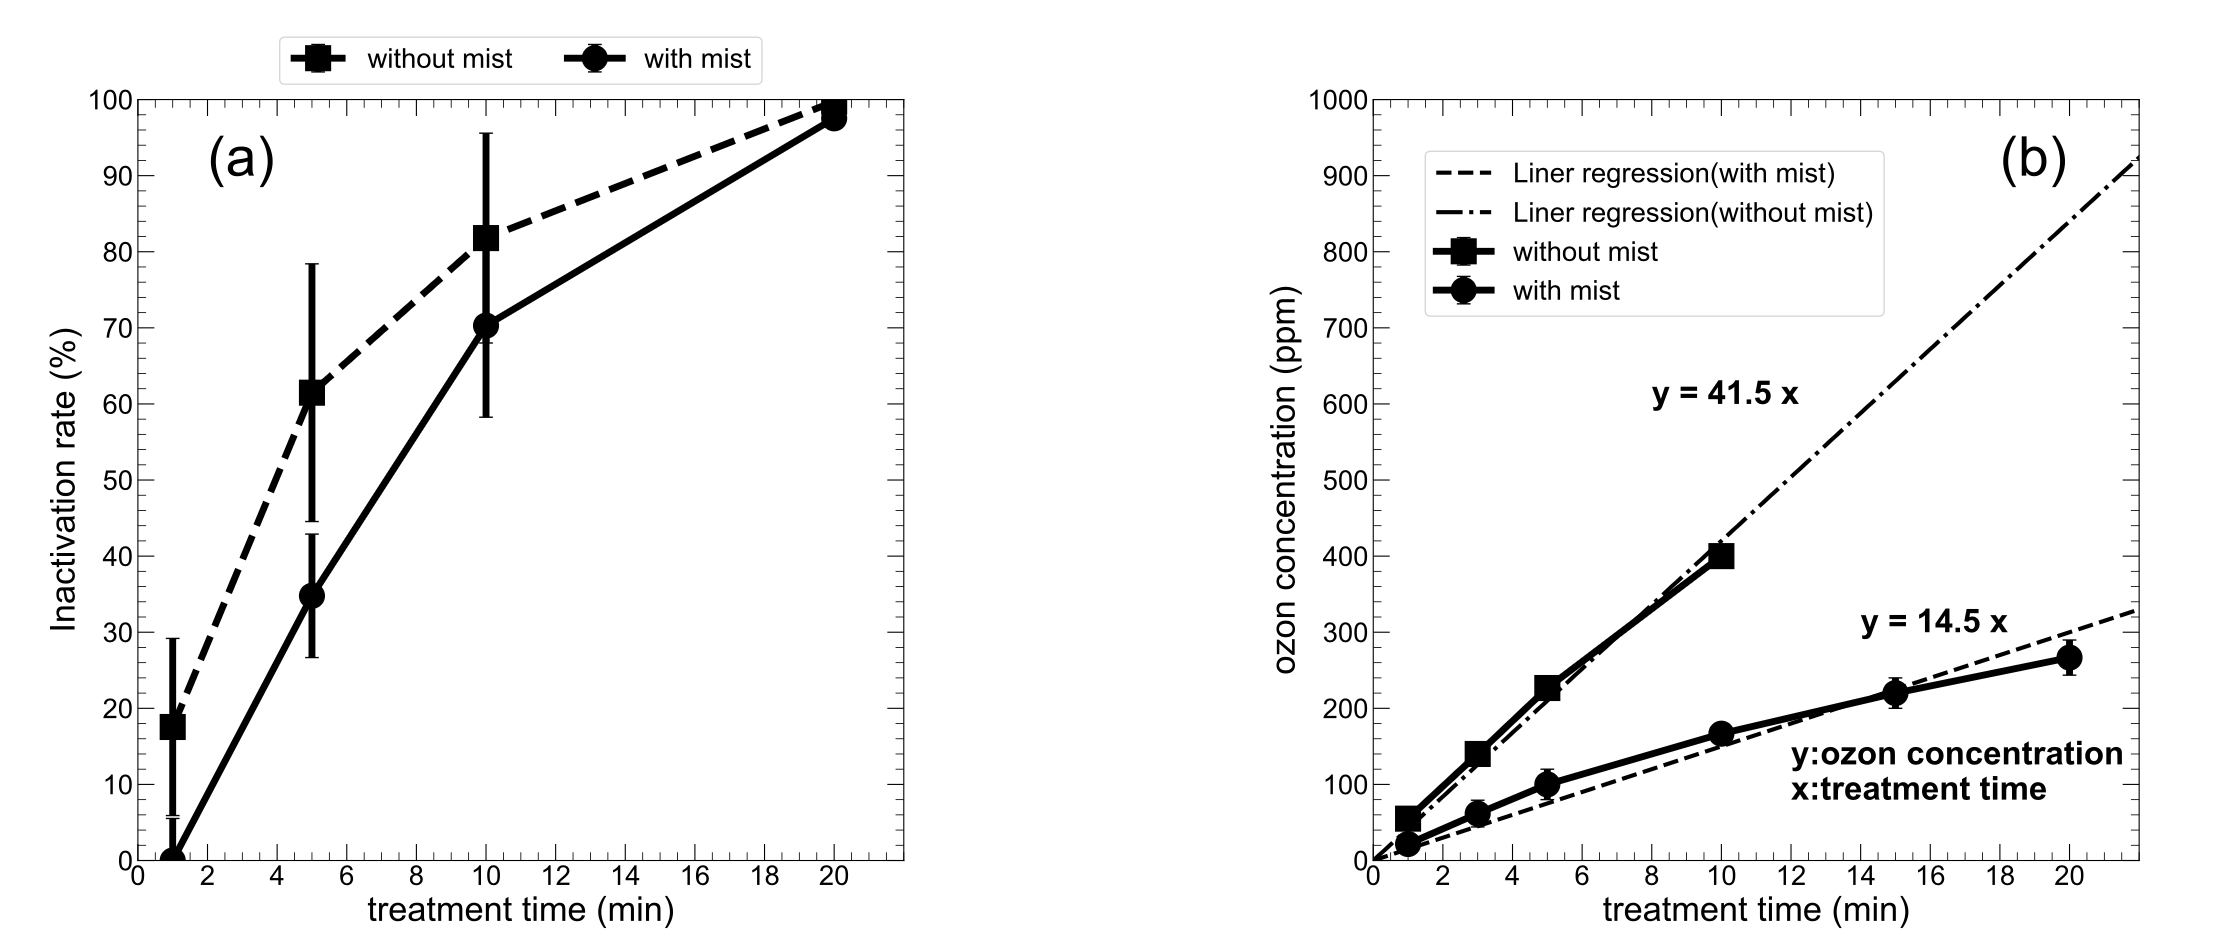
\includegraphics[width=1\textwidth]{images/KIT_work.png}
    \caption[Results of the study by Tomoya Ohara and others]{Results of the study by Tomoya Ohara and others \cite{kit}. (a) inactivation rates of C.sphaerospermum as a function of treatment time in the
    treatments without and with water mist, and (b) ozone concentration as a function of the
    time.}
    \label{fig:kit}
\end{figure}

\chapter{Theory and Methods}
\label{chap:theory}

In this chapter the theoretical background and the methods used in this work are presented. This includes the collection of research on the fungal species Cladosporium sphaerospermum, as well as the atmospheric pressure plasma and the different processes that lead to the sterilization of the mould as they interact. 

\section{Cladosporium sphaerospermum}
Cladosporium sphaerospermum (C. sphaerospermum) is a species of fungus. Fungi are a large group of eukaryotic organisms\footnote{Organisms whose cells have a membrane around their nucleus, which includes animals, plants and fungi.}  that include yeasts, moulds and common mushrooms. It is a black mould that is commonly found in indoor environments, especially in areas that are damp or have high humidity. It was first described by a German mycologist, Albert Julius Otto Penzig, in 1886 from decaying citrus plant material in Italy \cite{mould}. C. sphaerospermum primarily reproduces asexually through the production of conidia, which are non-motile spores\footnote{Spores not capable of movement.} formed at the tips of hyphae\footnote{Long, branching structures that grow from their tips. They give moulds their furry appearance.}. These spores are easily dispersed through the air, allowing the mould to rapidly spread into new environments. Moulds like C. sphaerospermum require humid conditions because moisture is essential for spore germination\footnote{The process by which a spore begins to grow new hyphae.}. In dry environments, spores usually remain dormant \cite{growth}.

\subsection{Growth and Morphology\footnote{The study of the structure of organisms.}}
C. sphaerospermum has a darkly-pigmented mycelium\footnote{A network of branching hyphae.} that can appear black or dark green. The colonies of the mould are typically flat and have more of a powdery appearance than other moulds. It is typical for fungi of the Cladosporium family to have branching, tree-like hyphae on whose ends conidia are formed in chains. The spores themselves are round to oval in shape and measure a few micrometers in length. They are very resilient and can stay alive even in conditions not favourable for growth. Due to their small size they are invisible to the naked eye. In Figure \ref{fig:mould} the morphology of C. sphaerospermum is shown. 

In addition to a humid environment optimal conditions for the growth of C. sphaerospermum include a temperature of 25  \textdegree C. It is however a  psychrophilic fungus\footnote{An organism that is able to grow in very low temperatures.} and can grow at temperatures as low as -5 \textdegree C \cite{mould}. It nourishes through saprotrophic nutrition, which is the process of using decaying or dead organic matter as a source of nutrients. This is why it is commonly found in decaying plant material, where it was also discovered. The conversion of starch, cellulose and other compounds such as carbon dioxide provides the energy needed for growth.

\begin{figure}
    \centering
    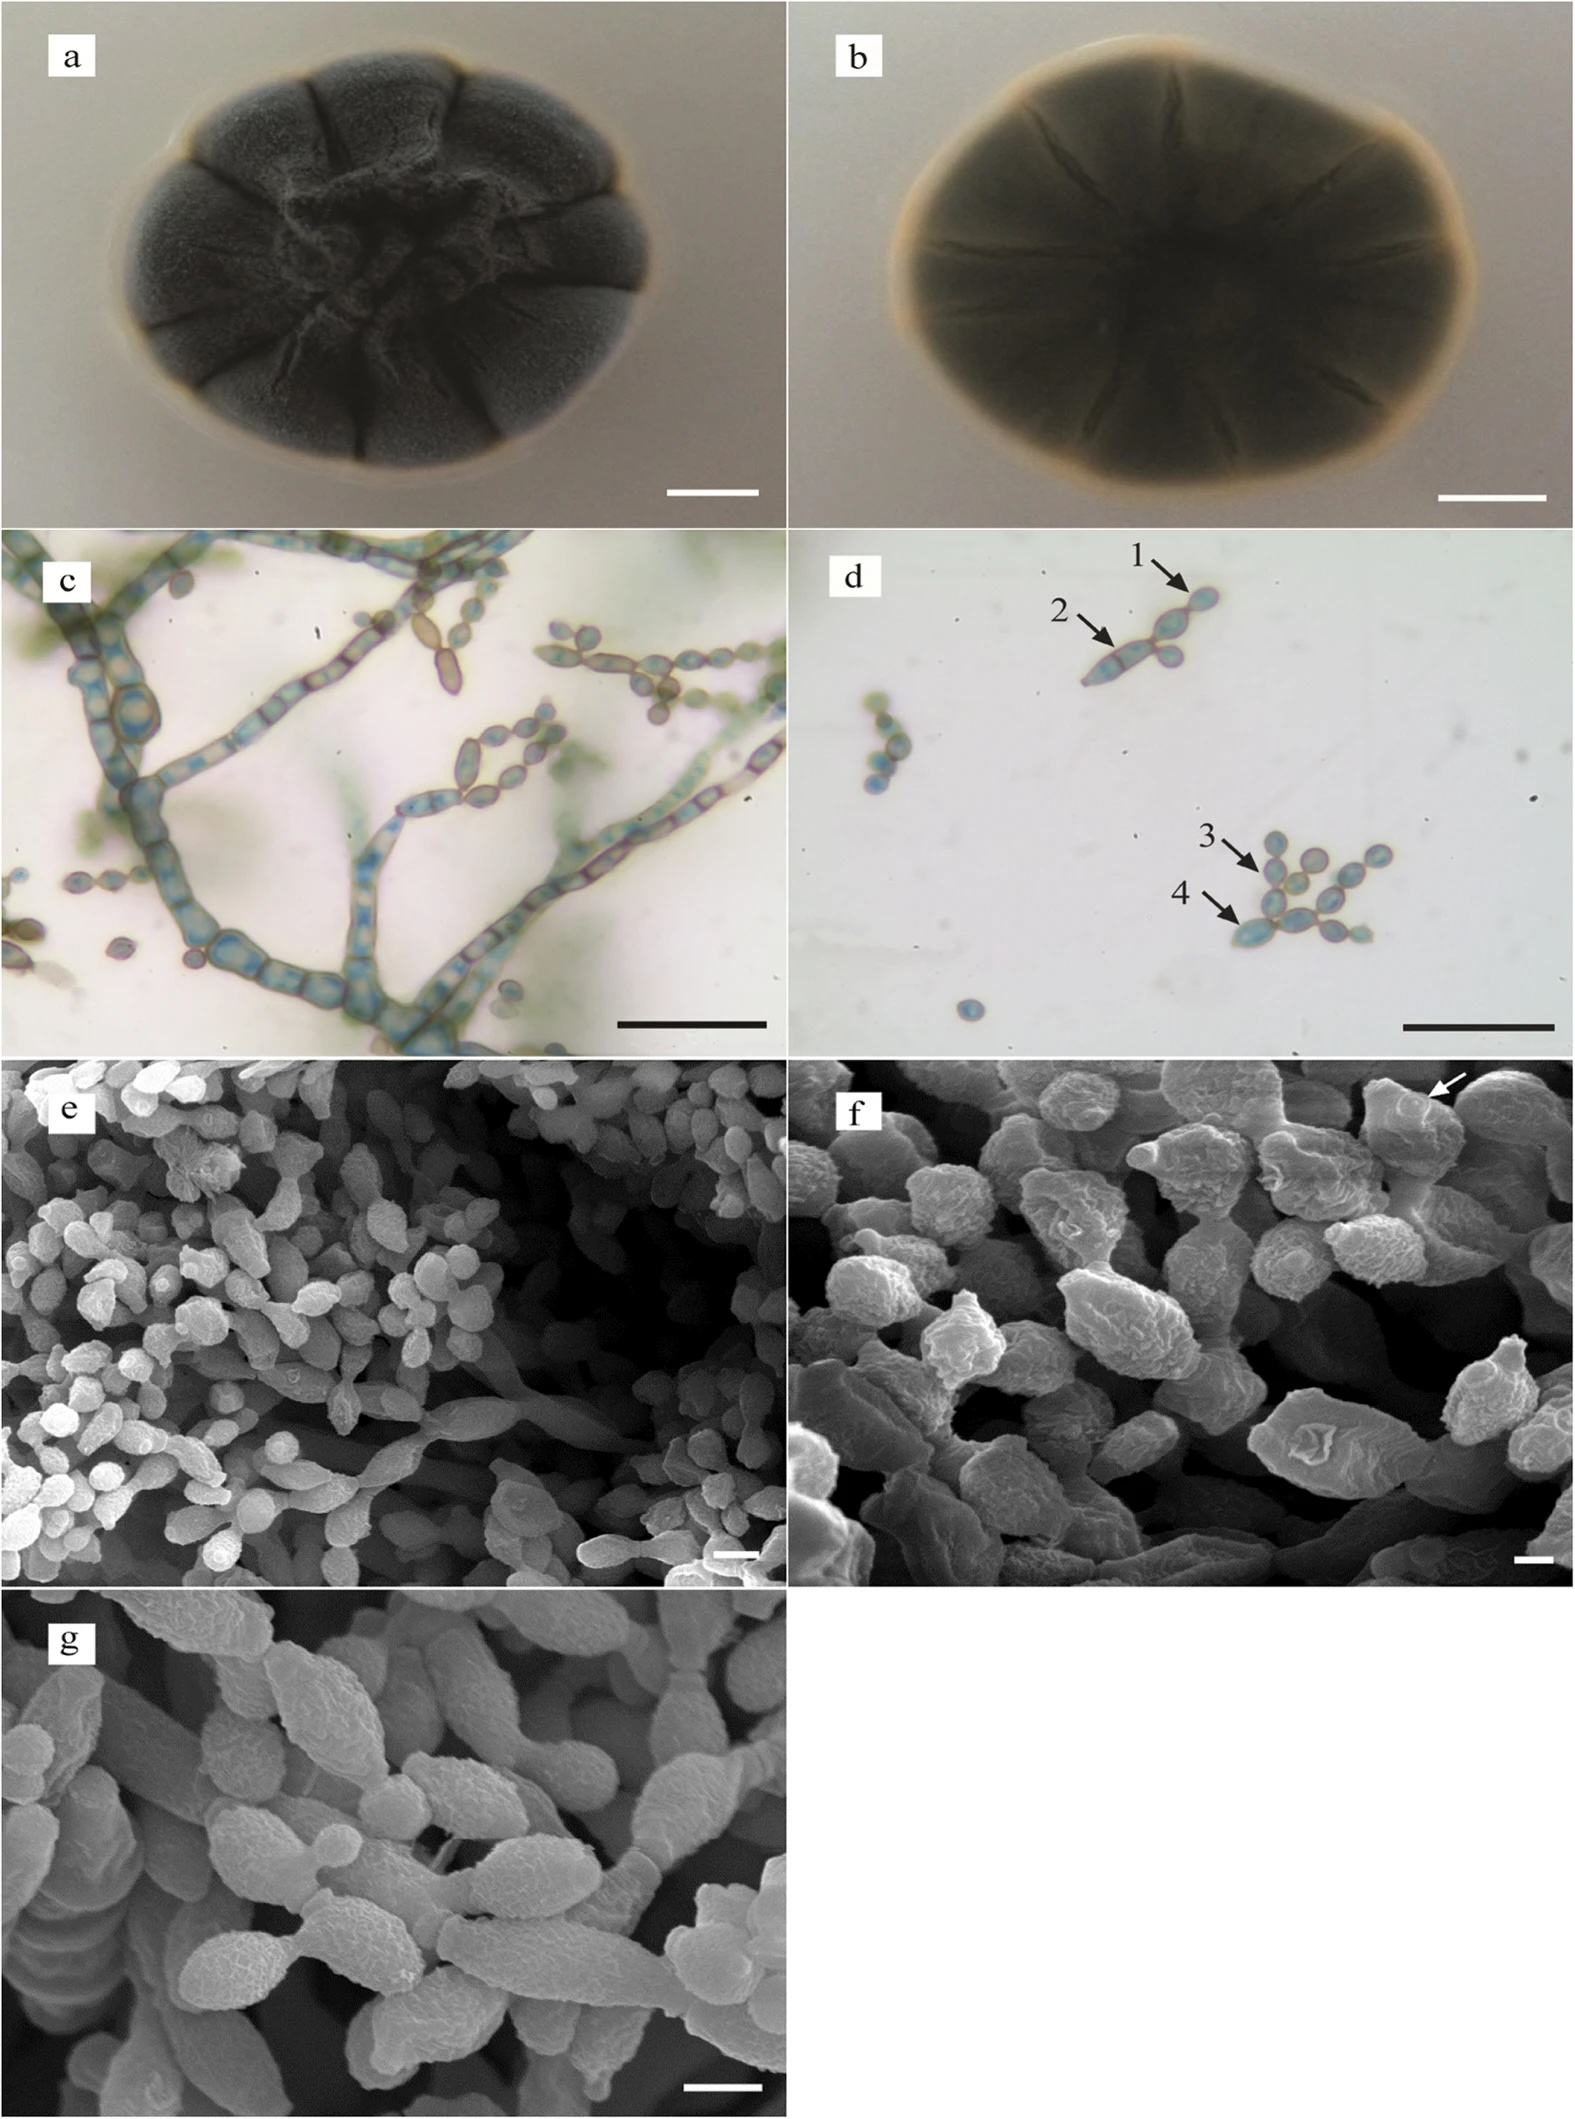
\includegraphics[width=.85\textwidth]{images/mould.jpg}
    \caption[Morphology of C. sphaerospermum]{Morphology of C. sphaerospermum from \cite{morphology}. Colonial morphology front (a) and reverse (b) of C. sphaerospermum UM 843 on SDA after 7-day incubation. Light micrograph showing conidia (d 2 and d 4). $\times$630 magnification, bars 20 \textmu m. Observation under scanning electron micrograph showing (e,f,g) conidiophores bearing conidium (e, $\times$2000 magnification, bar 3 \textmu m), periclinal rim\footnotemark. (f, $\times$5000 magnification bar 1 \textmu m) and verruculose surface of conidia (g, $\times$5000 magnification, bar 2 \textmu m).}
    \label{fig:mould}
\end{figure}

\subsection{Ecological Role and Occurrence}
Like many fungi C. sphaerospermum plays an important role in the ecosystem as a decomposer. It breaks down dead organic matter, recycling nutrients back into the soil, where it thrives. This process is important as it fertilizes the soil and allows for the growth of new plants, enabling the life cycle. Because of its resilience to different conditions it is able to grow in many different environments which include anthropogenic places like indoor environments. In humid areas and on porous surfaces, such as wood or concrete walls it can build mycelium and produce new spores. The easily dispersed spores reach virtually everywhere and are even found in orbiting spacecraft \cite{radiation}.

While fungi don't perform photosynthesis and therefore do not convert CO$_2$ into oxygen they still contribute to the carbon cycle. By digesting plant material and binding carbon dioxide in their biomass they play an important role in storing carbon and reducing the amount of carbon dioxide released into the atmosphere when plants decay. Because of there abundance they are able to store large amounts and help build stable compounds for long-term soil carbon storage.

\footnotetext{The outer edge of a cell wall layer formed parallel to the spore surface.}

\subsection{Effects on Human Health}
Because of its ubiquity C. sphaerospermum surrounds humans in their daily lives. The small size of the spores allows them to be inhaled deeply into the lungs where they can lead to allergenic reactions, as well as pathogenic infections\footnote{A pathogen is any organism that can cause disease in a host.}, particularly when the immune system is weakened. Compared to other airborne moulds it is however not considered a serious health risk as it does not produce mycotoxins\footnote{Toxins produced by certain fungi that can cause severe disease in humans and animals.}. Fungi in general can cause respiratory problems, especially when inhaling them in large quantities over a long time. They are however also essential in medical science as they are used to produce antibiotics, such as penicillin. While working with them in the lab clean benches can be used to provide sufficient ventilation but they generally don't pose any danger to a healthy person.

\subsection{Response to Radiation}
\label{sec:radiation}
UV radiation is commonly used to sterilize surfaces and is very effective in killing most microorganisms like bacteria and fungi. C. sphaerospermum however shows a higher resistance to different types of radiation including UV and even high energy ionizing radiation.  
It is able to not only survive doses of ionizing radiation that would kill most other organisms but also to thrive in these conditions. This was discovered in 1990s as the fungus is able to grow in the high radiation environment of the destroyed Chernobyl nuclear power plant \cite{radiation}, even on the highly radioactive reactor walls. The mould does not only survive in these conditions but was proposed to be radiotrophic - a process where fungi potentially use ionizing radiation as a source of energy analogous to photosynthesis - growing faster.

Its tolerance to radiation both ionizing and non-ionizing is attributed to the pigment molecule Melanin. Pigment molecules such as Melanin absorb visible light and other radiation which can protect cells, can be used to absorb energy. It gives the mould its dark colour and protects its from UV radiation. Melanin is also able to absorb ionizing radiation and potentially convert it into chemical energy usable to the fungus.

To further research this discovery the mould was sent to the International Space Station (ISS) in 2018 where it was exposed to cosmic radiation \cite{iss}. The study found that the mould was able to survive the radiation and even thrive in the microgravity environment while absorbing some of the energy. 

\subsection{Relation to Space Exploration}
Although it's not the main focus of this study, the connection of C. sphaerospermum to space exploration is briefly explored, as the author's university program focuses on space applications.

The study of fungi, like C. sphaerospermum, is not only interesting for terrestrial applications but also for use in space exploration. Because of its ability to survive in high radiation environments and the potential to use radiation as an energy source it might be useful in long-term space missions. NASA's Artemis program is currently the most prominent research projects that aims to send humans back to the Moon and eventually to Mars \cite{artemis}. This proposes many novel challenges surrounding the long-term survival and sustainability of human life in space. One of the biggest challenges is the radiation environment in space and on the moon, which is much harsher than on Earth. The radiation from cosmic rays and solar flares can cause severe damage to human cells and DNA, leading to cancer and other health problems \cite{shield}. The results of the study conducted on the International Space Station \cite{iss} suggest that C. sphaerospermum could potentially serve as a highly sought-after solution for creating a self-replicating biological radiation shield, as discussed in \cite{shield}. While shielding can be achieved with materials like polyethylene or aluminium, they are always a trade-off between weight and efficacy. Ideally, the shielding would be able to reproduce, be grown in situ and be combinable with on-site resources such as moon rock or soil \cite{shield}. This way, the shielding could be produced locally and would not need to be transported from Earth, making it possible to dramatically increase the thickness, as weight is not a concern. The use of radiotrophic fungi for this purpose still requires much more research, but the results of the study on the ISS are very promising.

The sterilization of surfaces in space is also a major concern. This is important for experiments to prevent contamination, especially those that involve taking samples from the surface of other celestial bodies. If it is possible to develop a portable plasma sterilization device using APPs, it might prove useful for on-mission sterilization of equipment and surfaces. This would be a great advantage over current methods that rely on chemicals or heat which are not always available or safe to use in spacecraft.

\section{Atmospheric Pressure Plasma}
A plasma is a state of matter that consists of ionized gas and free electrons. The particles behave collectively in a highly dynamic way because they are closely coupled  through electromagnetic fields. The state is also conductive, and the plasma can be influenced by external electric and magnetic fields \cite{plasma}. Although the particles carry charges locally, a plasma is electrically neutral when observed as a whole. Plasmas can be created by applying energy in the form of heat or electromagnetic fields to a gas. To ignite a plasma at low temperatures, a discharge is needed, the conditions for which - such as pressure, voltage and distance - are described by Paschen's law. This law states that it is generally easier to create a plasma in a low-pressure environment, as the mean free path (the distance between particle collisions) is larger, allowing the electrons to gain more energy before colliding with other particles, so they can exceed the ionization threshold. This is why many plasmas are created in vacuum chambers. However, with a sufficiently high voltage, it is  possible to create plasma at atmospheric pressure also. Such a plasma is known as an atmospheric pressure plasma (APP). APPs have the advantage of being comparatively simple to handle as no vacuum vessel is required to contain them. This also makes it easier to bring them into the proximity of samples for various applications such as sterilization, surface treatment or material processing \cite{plasma}. To sustain the plasma an alternating current in the Kilohertz range is used, so that the changing electromagnetic field is able to accelerate electrons continuously. The much heavier ions are accelerated only minimally in comparison. Although electron temperatures commonly reach around 10$^4$ K, it is possible to sustain a plasma at room temperature if the energy provided is controlled \cite{plasma2}. Such plasmas are referred to as cold plasmas or non-thermal plasmas. Because of the high voltage required to ignite APPs arc discharges can occur between the electrodes which significantly reduce the plasma stability. This makes it very hard to predict their behaviour and would heat them up to much higher gas temperatures which needs to be prevented for many experiments. Dielectric barriers can be used to achieve a controlled discharge and energy transfer. 

Many processes occur in a plasma besides ionization. The gas atoms are also frequently excited which leads to the emission of photons as these states are non-stable which gives plasmas their characteristic glow. Molecules can also be dissociated by collisions which leads to the formation of radicals and other chemical bonds that can have varying lifespans. The radiation, as well as the reactive species produced in the plasma, allows the plasma to interact with surfaces and materials in its proximity.

\section{Dielectric Barrier Discharge}
To achieve a controlled non-thermal plasma at atmospheric pressure a dielectric barrier discharge (DBD) can be used. This means that the two electrodes that carry the high voltage to ignite and sustain the plasma are separated by a dielectric barrier. There are different configurations to realize this. Some setups use only one dielectric barrier at one of the electrodes, while commonly both electrons - planar or cylindrical - are covered with a dielectric material. The dielectric barrier is a non-conductive material that prevents the formation of an arc discharge between the electrodes, but can be polarized by the electric field. Often glass, quartz or ceramics are used for this purpose. While the plasma is ignited, the dielectric barrier prevents the electrons from flowing freely between the electrodes and charges are built up on the surface of the dielectric. This stops the discharge very quickly and thereby limits the current flow, an alternating current is needed to sustain the discharge. By controlling the voltage and frequency of this current the discharge can be sustained in a stable way. The dielectric barrier also helps to create a uniform electric field, similar to its use in capacitors. 

DBD is used widely in different applications that require a non-thermal plasma like the semiconductor or medical industry. It is used for surface treatment, cleaning and sterilization, like in this work, where a cold plasma is needed that does not destroy the surfaces it interacts with.

\section{Optical Emission Spectroscopy}
Optical emission spectroscopy (OES) uses the electromagnetic radiation emitted by a plasma to analyse its composition. This can be done non-intrusively, meaning that the plasma does not need to be disturbed and remains unaffected by the measurement. That is a major advantage when working with small volumes of plasma, like in this work, where probes would significantly change the conditions \cite{plasma2}. OES measures a spectrum of the emitted light which gives the intensity at different wavelengths. Because the photons originate from distinct transitions between energy levels, sharp peaks are observed in the spectrum. Their wavelength can be used to identify the species that are present in the plasma, as well as the processes that occur. This also allows an estimate of the plasma temperature and the concentration of the different gases in the plasma, although more information, like cross-sections for the different processes, is needed \cite{plasma2}. 

In OES one needs to account for the spectrometer's spectral response, which is the sensitivity of the detector per wavelength. This is usually done by measuring a calibration spectrum and correcting the measured spectrum accordingly.

\subsection{Boltzmann Plots}
\label{sec:boltzmann}
Boltzmann Plots are often used to derive the electron temperature $ T_\text{e} $ from a measured spectrum. They underlie the assumption that the probability for transitions follows a Boltzmann distribution, with the intensity of the emission line proportional to the Einstein coefficient for spontaneous emission. The relationship between intensity and temperature is given by:

\begin{equation}
    \frac{I_j}{g_j} \propto A_{ij} \exp\left( - \frac{E_j}{k_\text{B} T_\text{e}} \right),
\end{equation}

where $ I_j $ is the intensity of the emission line from an excited state $ j $, $ g_j $ is the degeneracy of that state, $ E_j $ is the energy of the state, $ A_{ij} $ is the Einstein coefficient for spontaneous emission, and $ k_\text{B} $ is the Boltzmann constant. 

When the intensities are put in relation in a plot of $ \ln \left( \frac{I_j}{g_j A_{ij}} \right) $ over the energy $ E_j $ they result in a straight line. The slope $ m $ of this line provides an estimate for the electron temperature $ T_\text{e} $:

\begin{equation}
    m = - \frac{1}{k_\text{B} T_\text{e}}.
\end{equation}

However, it is also assumed that the plasma is in local thermal equilibrium which is not the case in non-thermal plasmas. The assumption that the electron temperature is equal to the gas temperature is not valid and the Boltzmann plot can not be used to get an absolute temperature value in this work \cite{plasma2}. 

\subsection{Other methods}
\label{sec:oes_temperature}
A very interesting study by Hiroshi Akatsuka \cite{oes_temperature} was able to show that the electron temperature and density can be derived from the OES spectrum of a non-equilibrium plasma. To do so the continuum spectrum of the plasma was measured and its absolute emissivity per wavelength $\lambda$ was calculated. The continuum spectrum is caused mainly by \textsc{Bremsstrahlung} emitted by decelerating electrons in the plasma \cite{oes_temperature}. It is much less intense than the peaks formed by electron transitions but is closely related to the electron temperature and density. The following relationship describes how the emissivity $\varepsilon_\lambda$ and the intensity $I_\lambda$, found through OES, are related and the optical length through the plasma $L$ is known:
\begin{equation}
I_\lambda = \int_0^L \varepsilon_\lambda(l) \, dl.
\end{equation}
By then fitting an electron energy distribution function (EEDF) to the measured spectrum the electron temperature and density can be derived as fit parameters. The EEDF describes the distribution of the electron energy in the plasma and is a function of the electron temperature. A Maxwellian distribution and a Druyvesteyn distribution were used in the study to obtain accurate results \cite{oes_temperature}. While the results from this study are used as a reference for comparison the method itself could not be applied in this work because of limited resources and time.  

\section{Sterilization Mechanism}
APPs have been used for sterilization of surfaces in many studies as outlined in chapter \ref{chap:scientific_context}. Although the plasma is not in direct contact with the sample two main mechanism have been found to be responsible for the sterilization effect. The first is the radiation emitted by the plasma, which can be UV or visible light. The second is the reactive species that are produced in the plasma and interact with the surface. Additionally, heat, as well as electric fields, can also play a role in the sterilization process. The exact mechanism is still subject to research and what process dominates depends on the specific setup and sample. This study aims to test and isolate the effects of the radiation and reactive species on the inactivation of C. sphaerospermum. The following sections will discuss what is known about the different processes and how contribute to the sterilization.

\subsection{Reactive Species}
As discussed in chapter \ref{chap:scientific_context} the main mechanism for the inactivation of microorganisms in prior studies appeared to be the reactive species produced in the plasma. Because of the high electron temperatures in the plasma some electrons gain enough energy to dissociate molecules and create radicals. When working with an APP using air the main gases present are oxygen and nitrogen, as well as water vapour. The most important reactive species produced are hydroxyl radicals (OH) and ozone (O$_3$). Radicals are missing an electron and are therefore highly reactive chemicals. They are widely used in water treatment and sterilization, because they can react with organic compounds and degrade them \cite{water}. Studies such as \cite{ozone} have demonstrated that the concentration of ozone can be correlated with the rate of microbial inactivation directly. These reactive species can penetrate cells and cause damage to vital biomolecules, including DNA and proteins.
This leads to the inactivation of the microorganism as it is unable to reproduce or perform its normal functions and was proven to be effective against the spores of C. sphaerospermum \cite{kit}. By using chemical probing methods the concentration of reactive species can be measured. For example the concentration of OH radicals can be quantified by their fluorescence when they are reacted with a chemical probe such as sodium terephthalate (NaTA). 

\subsection{Radiation Effects}
In addition to the radicals produced by the plasma it emits radiation that interacts with the sample. In APP visible light, as well as UV light in the UV-A and UV-B range, is typically emitted \cite{plasma2}. UV radiation is used a lot for sterilization and is standard in many clean benches used in laboratories but slightly higher frequencies in the UV-C range are used. A study by Li, Yiqian and others \cite{bacteria} found that plasma emitting UV-A and UV-B light can have a significant effect on the inactivation rate of bacteria when using a quartz-glass separation but that the shorter wavelengths are more effective.

The main reason why UV radiation is effective at killing microorganisms is its photochemical interaction with DNA. DNA is very susceptible to absorption of UV light, which can alter its structure leading to the breaking of bonds and the formation of mutations \cite{DNA}. DNA contains four bases: adenine (A), thymine (T), cytosine (C), and guanine (G). These are all aromatic molecules. Aromatic molecules are ring-shaped compounds with delocalized \text{$\pi$-electrons}, meaning their electrons are not confined to individual bonds but can move freely within the molecule \cite{DNA}. This makes them highly stable, but the electrons can efficiently  be excited by  UV light, especially around 260 nm. The transition \begin{equation}
    \pi \rightarrow \pi ^\star,
\end{equation}
describes the excitation of an electron from a bonding\footnote{A bonding orbital results from constructive interference of atomic orbitals, lowering electronic energy.} $\pi$-orbital to an anti-bonding\footnote{An anti-bonding orbital results from destructive interference of atomic orbitals, raising electronic energy.}  $\pi^\star$-orbital. This significantly weakens the bonds in the molecule and can lead to the formation of dimers\footnote{In DNA, dimers can form when two adjacent bases bond abnormally due to UV exposure \cite{DNA}.}. Fungi, just like bacteria, rely on the integrity of their DNA, as it is the basis for their reproduction of cells, which makes any damage to the DNA highly effective in killing them.

As mentioned in section \ref{sec:radiation} C. sphaerospermum is more resistant to UV radiation than bacteria because it is a melanized fungus. Melanin helps to protect the DNA from UV radiation by absorbing some photons before they reach the DNA. This means higher doses are necessary to achieve the same inactivation rate.
\chapter{Experimental Setup}
\label{chap:experiment}

\section{APP Setup}

\begin{figure}
    \centering
    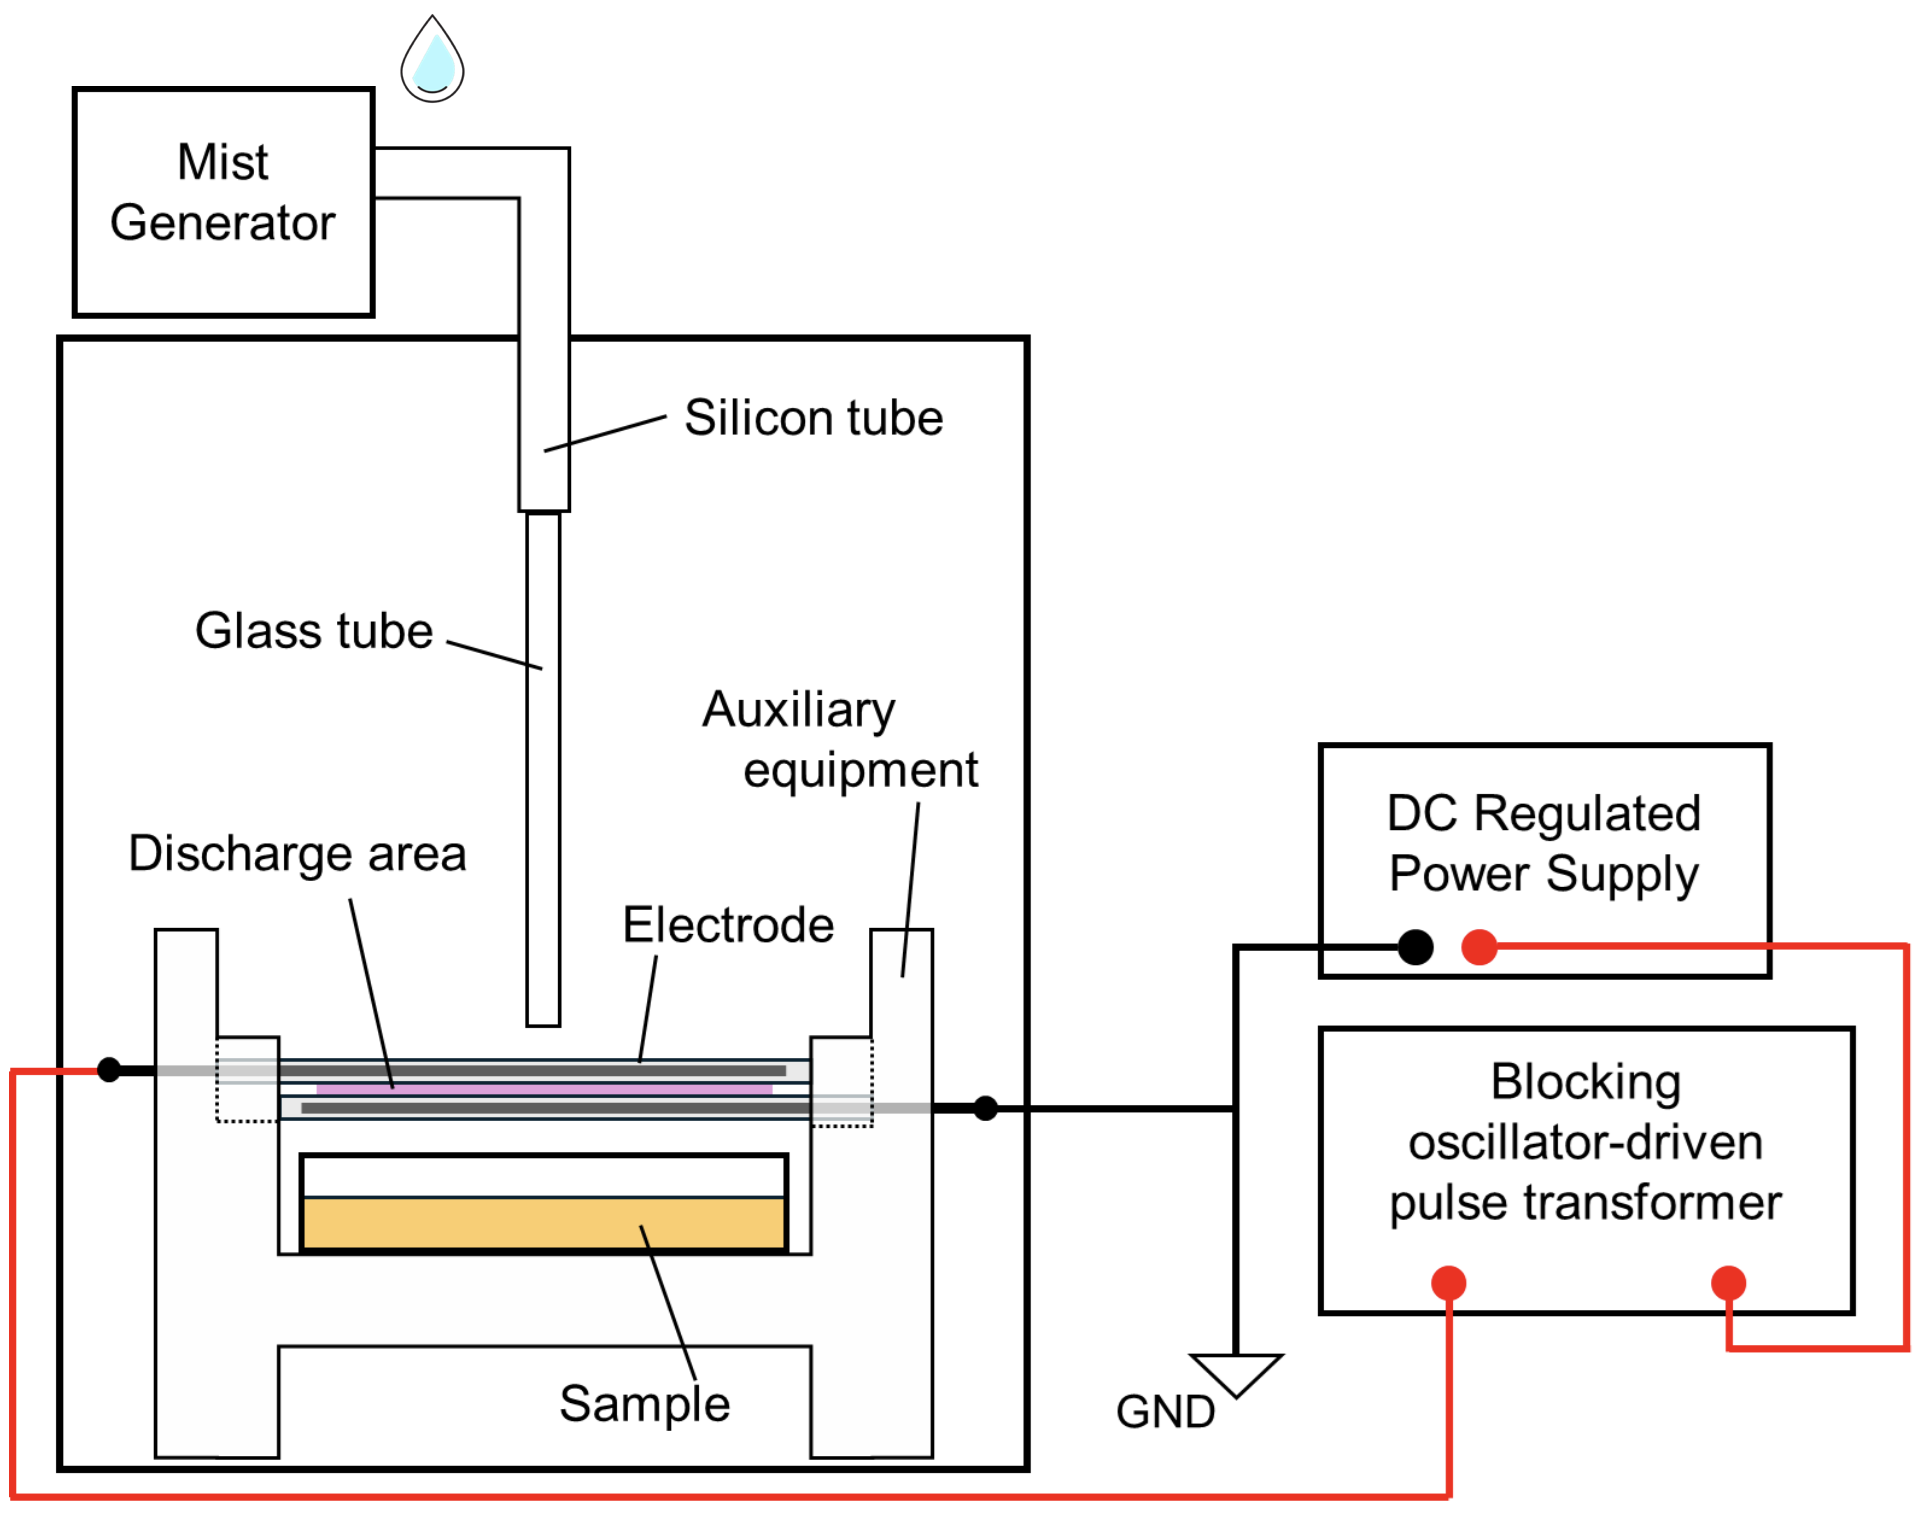
\includegraphics[width=1\textwidth]{images/Process_setup.png}
    \caption[Experimental setup]{This figure shows the experimental setup. The APP is generated between two pairs of electrodes. The entire setup is placed in a box to prevent contamination. The sample is placed underneath the discharge area. A tube can provide water mist and dry air to control the humidity in the chamber. A power supply and a blocking oscillator provide an oscillating voltage to the electrodes.}
    \label{fig:setup}
\end{figure}

\subsection{Dielectric Barrier Discharge}
\begin{figure}
    \centering
    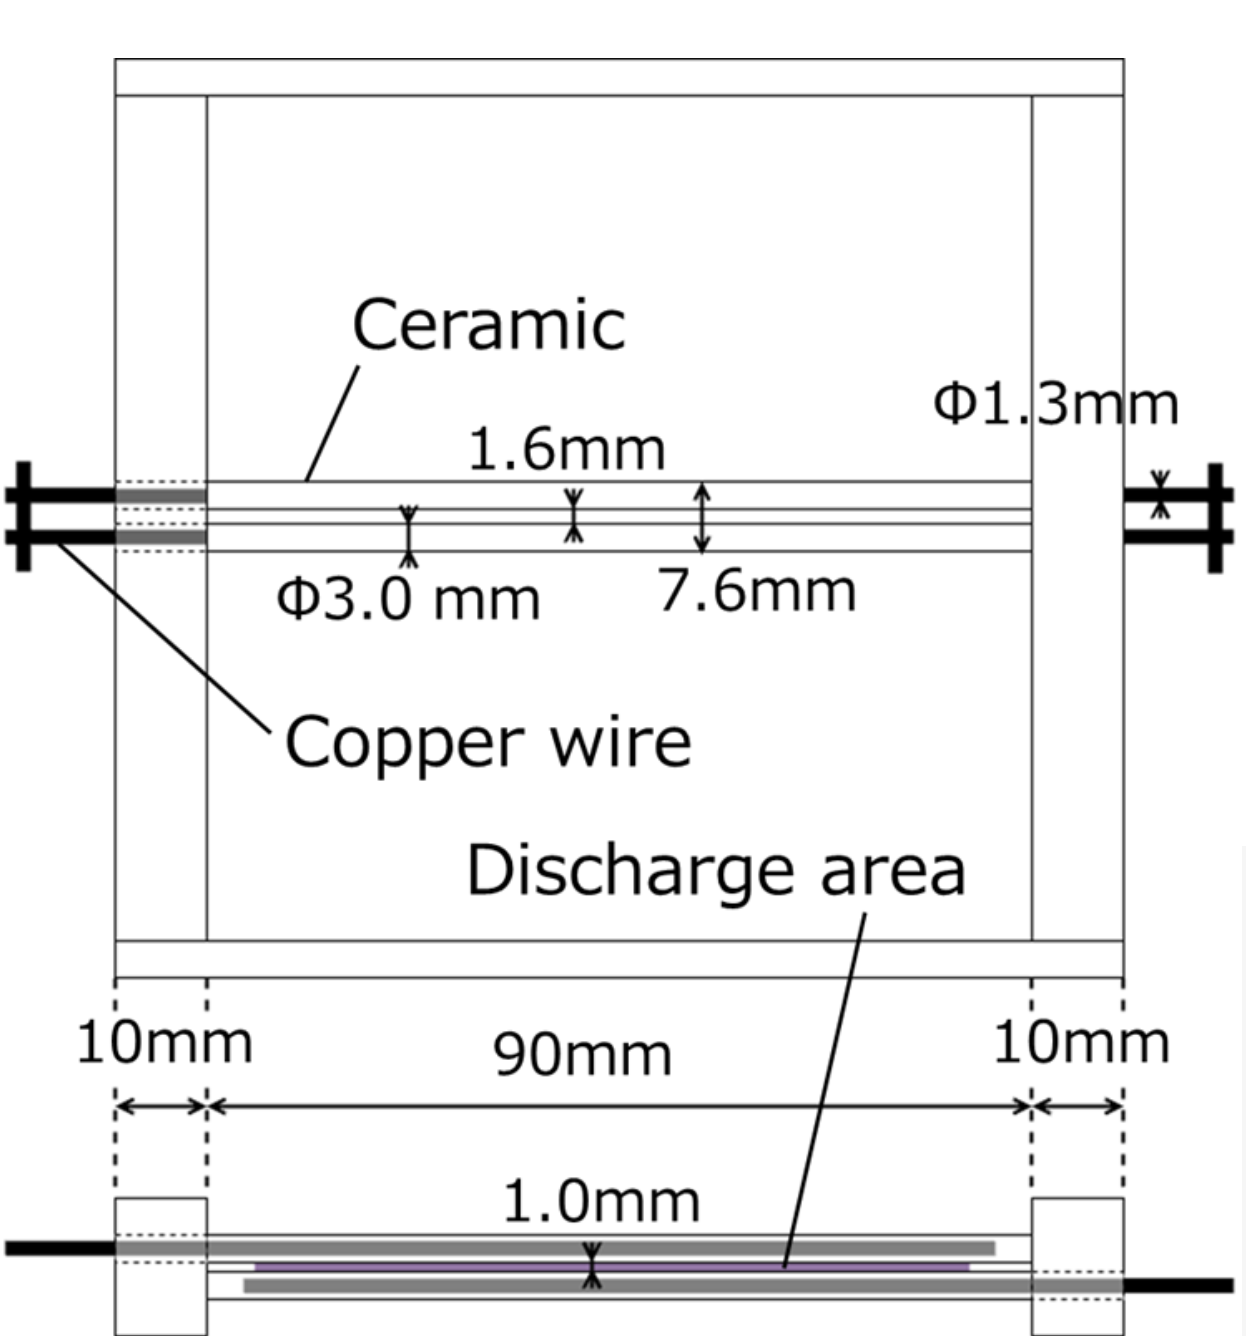
\includegraphics[width=.8\textwidth]{images/APP_setup.png}
    \caption[Technical sketch of the DBD setup]{Technical sketch of the DBD setup. On the top the view from above the DBD setup is shown, on the bottom the side view. The APP is generated by a DBD with a frequency of 13.56 MHz and a voltage of 13 kV. This diagram has kindly been provided by Shinano Kinoshita at KIT.}
    \label{fig:dbd}
\end{figure}

\begin{figure}
    \centering
    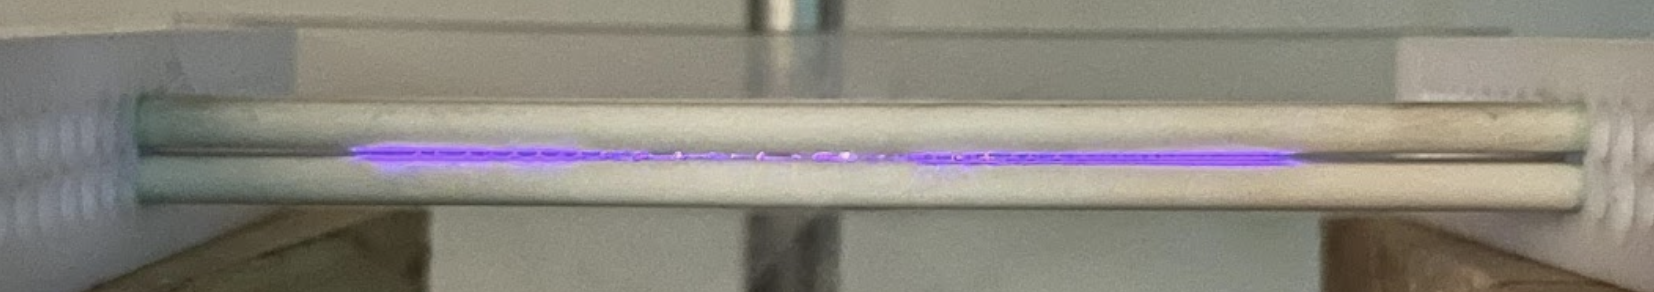
\includegraphics[width=1\textwidth]{images/Plasma.png}
    \caption[Image of the APP]{Image of an ignited plasma at atmospheric pressure between the electrodes.}
    \label{fig:plasma}
\end{figure}


\subsection{Optical Emission Spectroscopy}

\section{Preparation of Samples}
\begin{figure}
    \centering
    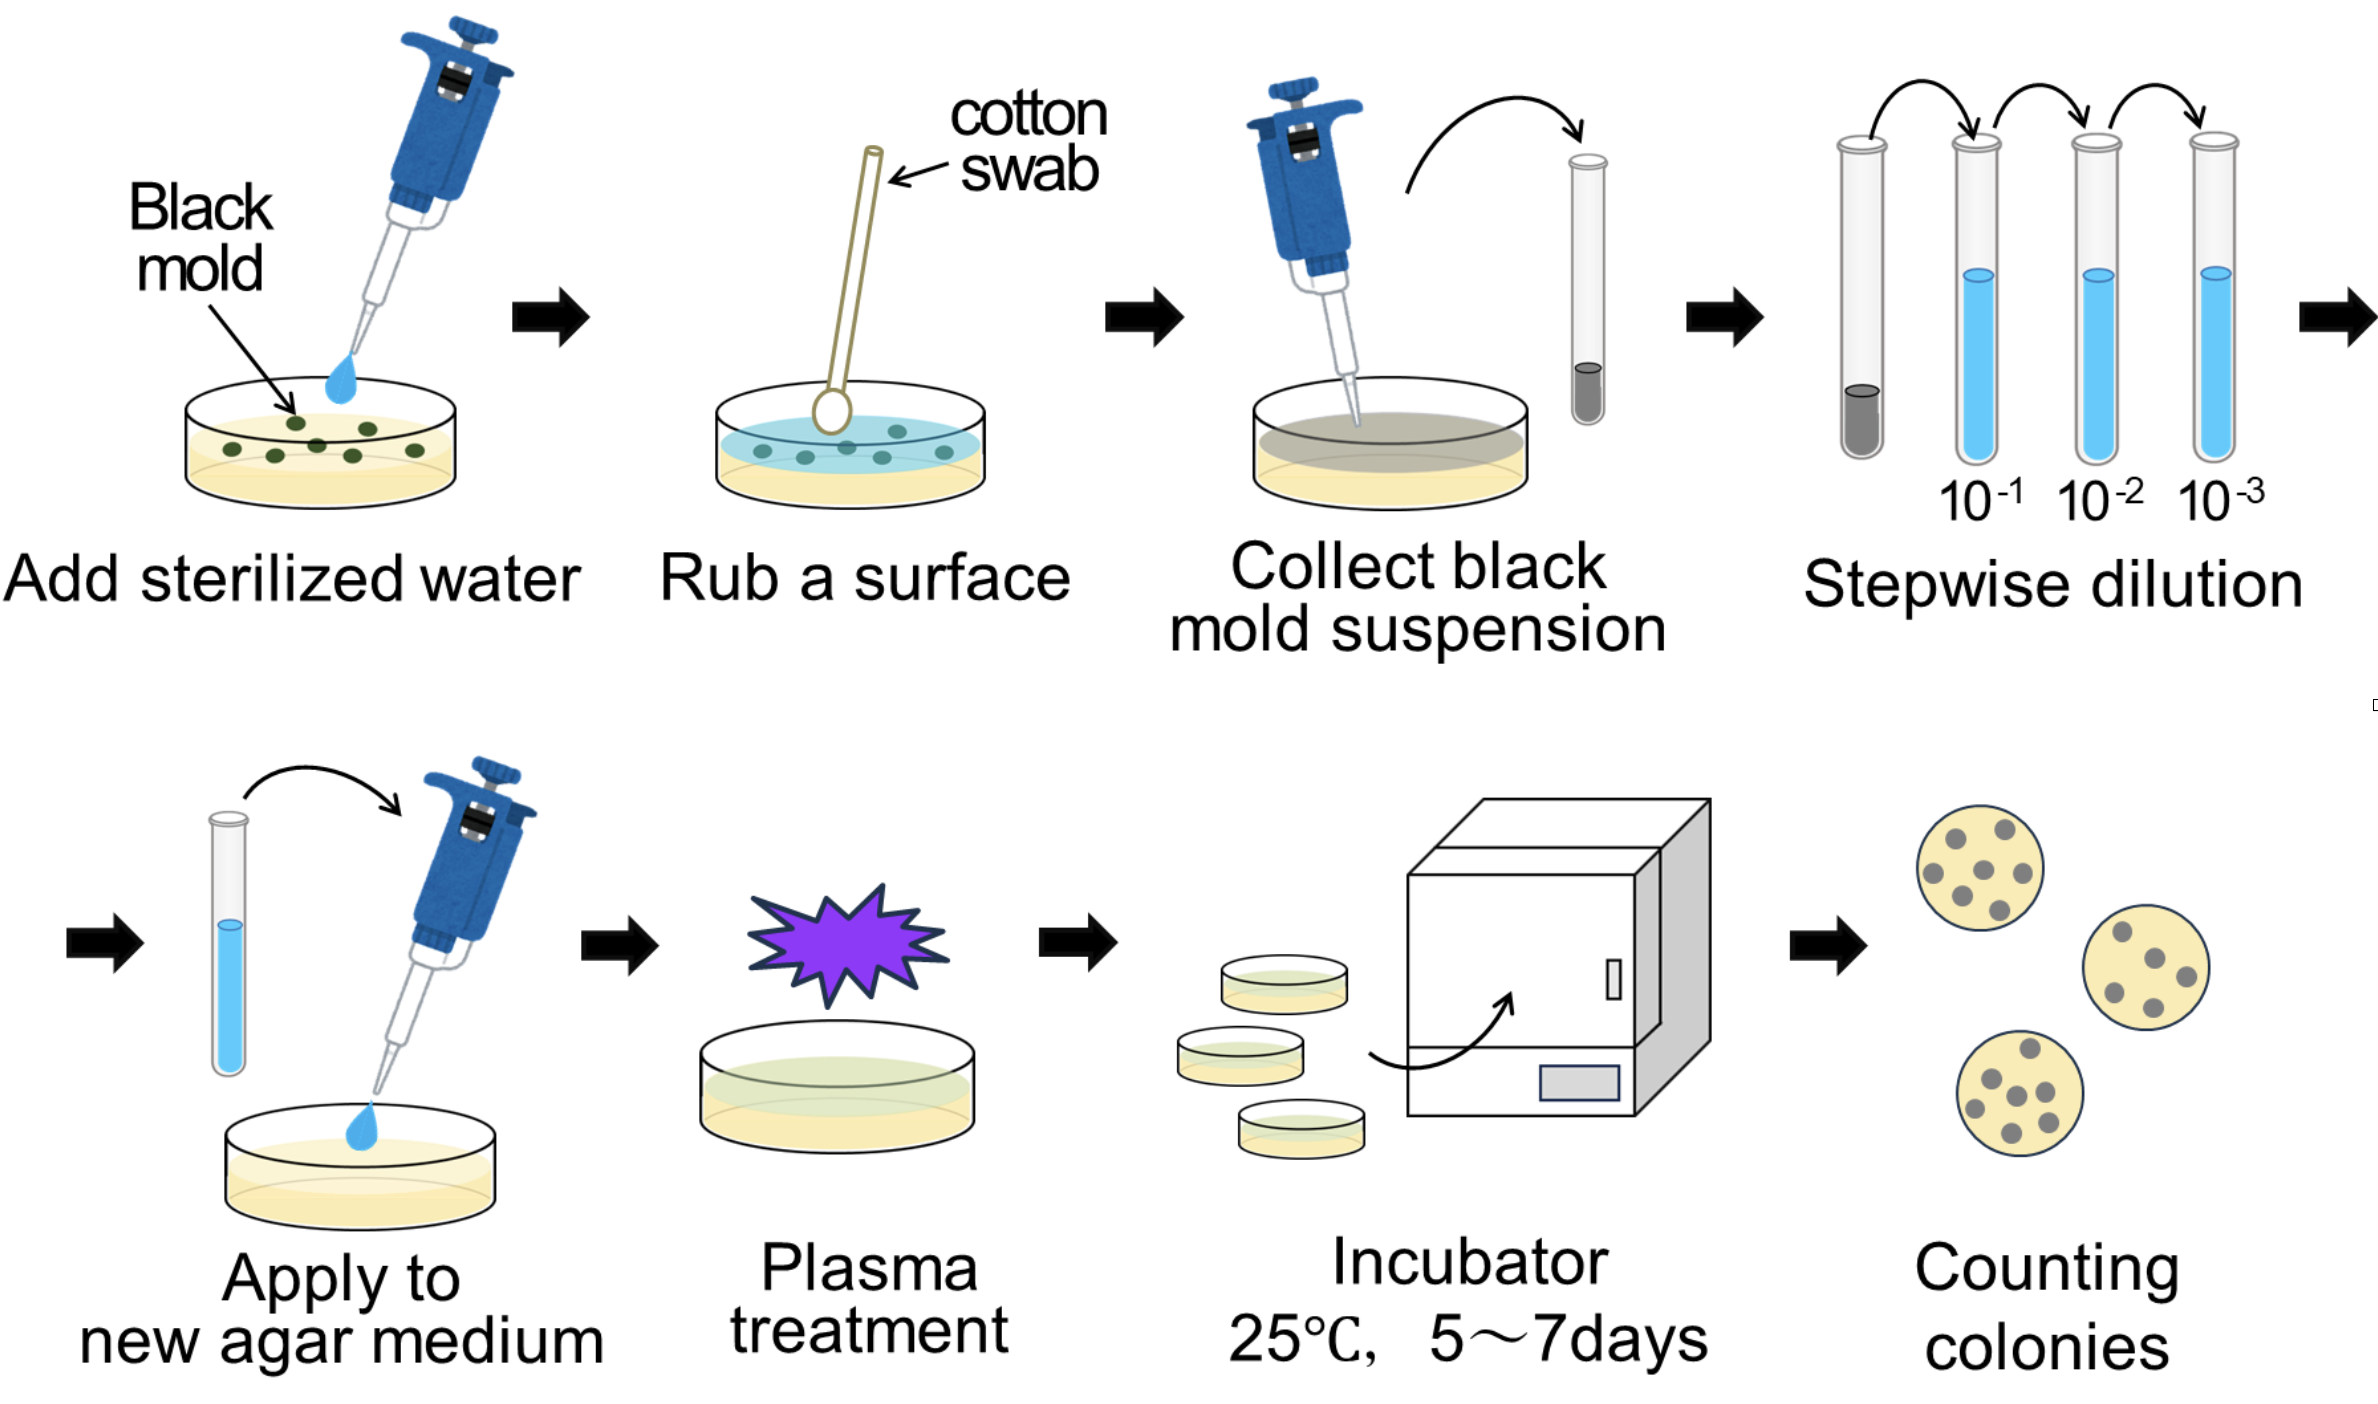
\includegraphics[width=1\textwidth]{images/Process.png}
    \caption[Diagram of the experiment process]{Diagram of the experiment process and the preparation of samples. The fungus is cultivated on an agar medium and stored in petri dishes. Spores are collected by dissolving them in sterilized water and then their concentration is diluted in steps to the desired concentration. The samples are then treated with the APP and the inactivation rate is measured by counting the colonies on the agar medium.}
    \label{fig:process}
\end{figure}

\section{UV Exposure}

\section{Plasma Treatment}

\subsection{Full Plasma Treatment}
\subsection{Isolation of Radiation}



\chapter{Results}
\label{chap:results}
In this chapter the results of the experiments are presented. They are divided into three sections that were conducted consecutively to answer the research question that were posed in the introduction. The first section shows an analysis of the OES spectrum of the APP and confirms the plasma composition. The second section describes the effect of UV radiation had on the spores of C. sphaerospermum in the experiment. In the third section results of the APP treatment on the spores of C. sphaerospermum with and without reactive species are shown. 

\section{OES Analysis}
\label{sec:oes_analysis}
In the following the OES spectrum of the plasma first shown in section \ref{sec:oes} is analysed. To do so, the peaks of the spectrum are found using \textsc{Python} and the \textsc{SciPy} library. They are then compared to possible different species that could be present, and their wavelengths matched to identify the transitions. Figure \ref{fig:oes_analysis} shows the spectrum with the peaks marked using \cite{nist, spectra, spectrum}. The spectrum confirms the presence of the main species in the plasma, which are as expected mostly nitrogen, oxygen and water. Most oxygen is dissociated and makes new compounds with hydrogen or nitrogen leaving nitrogen molecules to be dominant in emission. Almost all visible peaks were found to correspond to the Second Positive System (2PS) of nitrogen. The 2PS is a system of transitions between the vibrational levels of the first excited state of nitrogen:
\begin{equation}
    \mathrm{N_2\ C^3\Pi_u \rightarrow B^3\Pi_g}
\end{equation}
and consists of many bands. Figure \ref{fig:n2_2ps} shows a plate of the 2PS of molecular nitrogen.


\begin{figure}
    \centering
    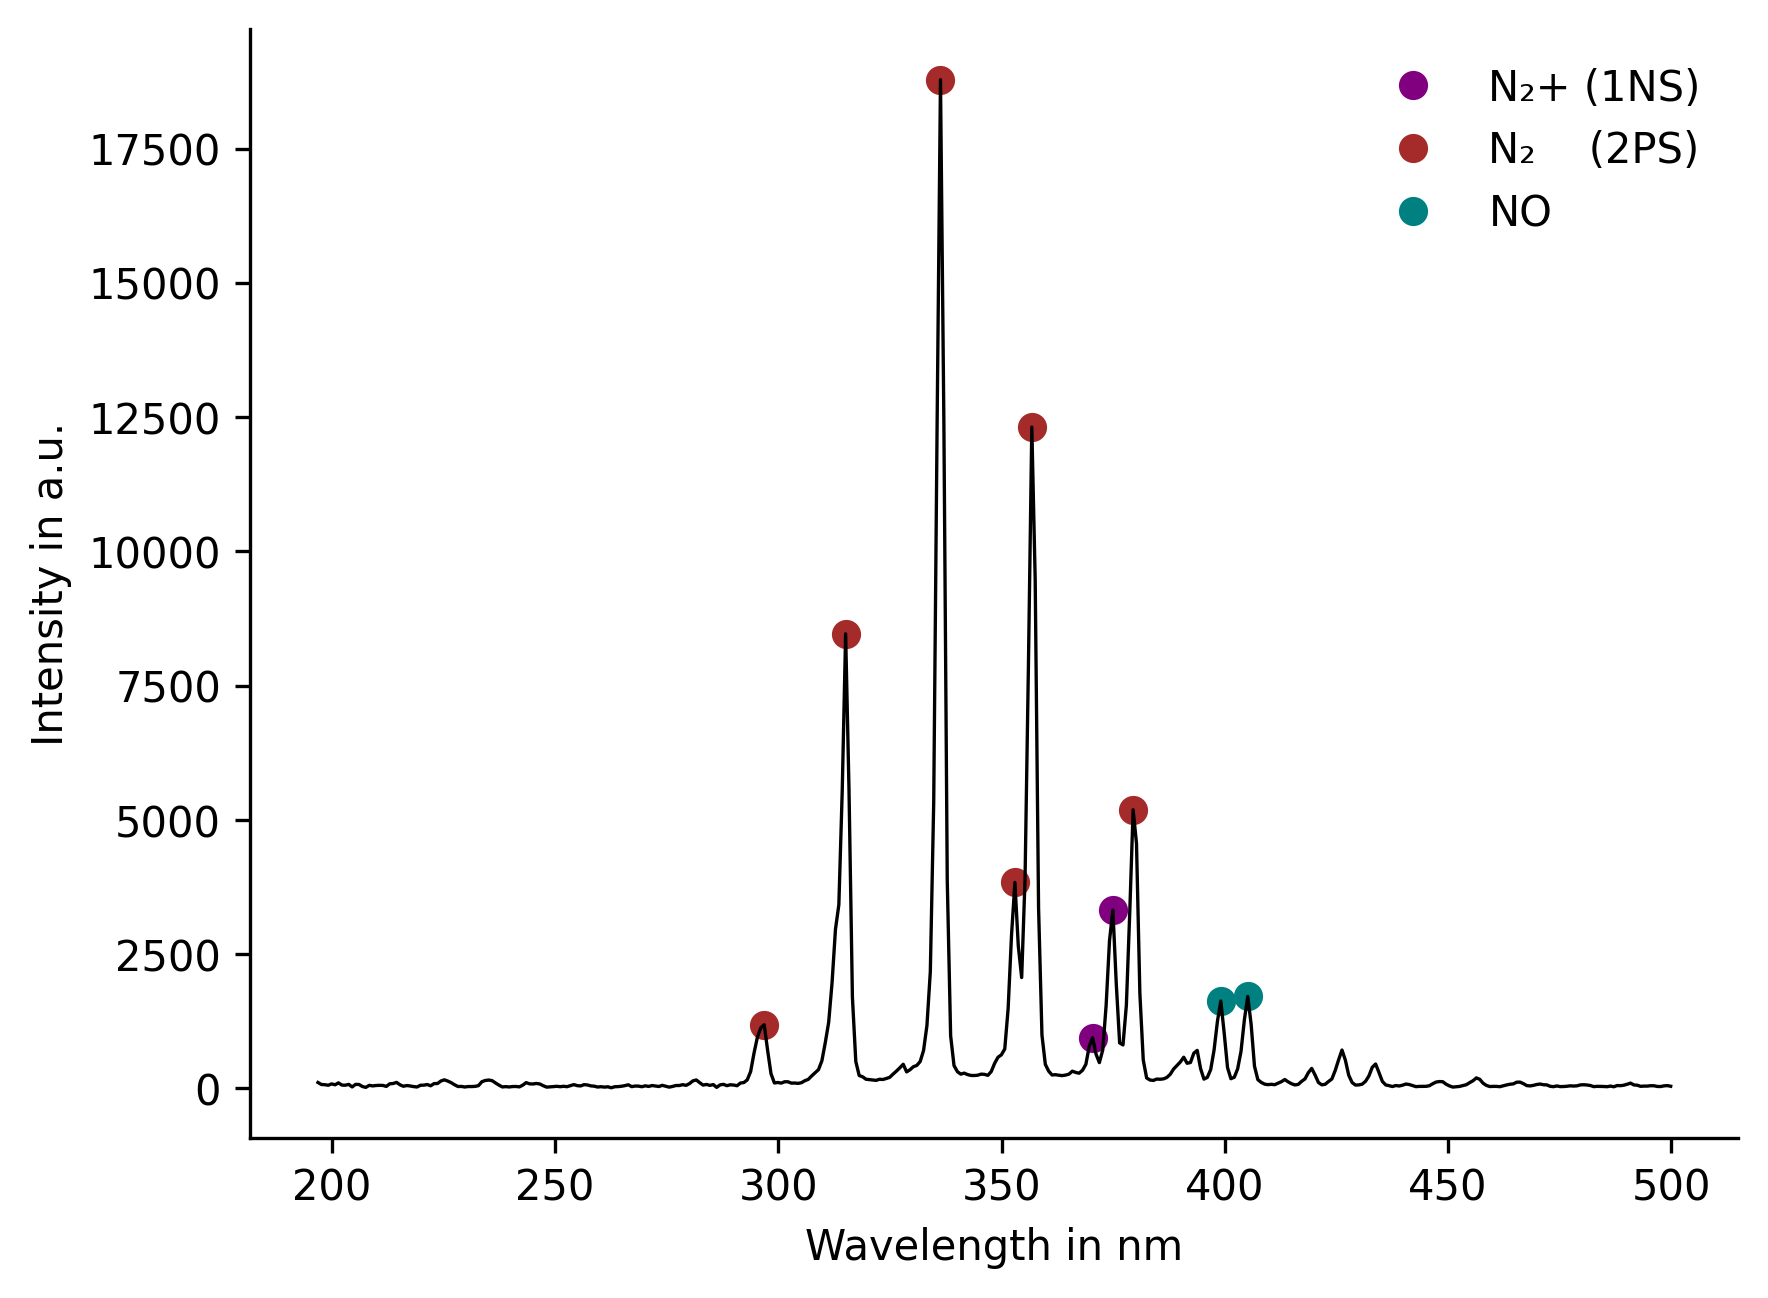
\includegraphics[width=1\textwidth]{images/OES_analysis.png}
    \caption[OES spectrum with identification]{OES spectrum of the plasma with the peaks identified. The Second Positive System of molecular nitrogen is dominant.}
    \label{fig:oes_analysis}
\end{figure}

\begin{figure}
    \centering
    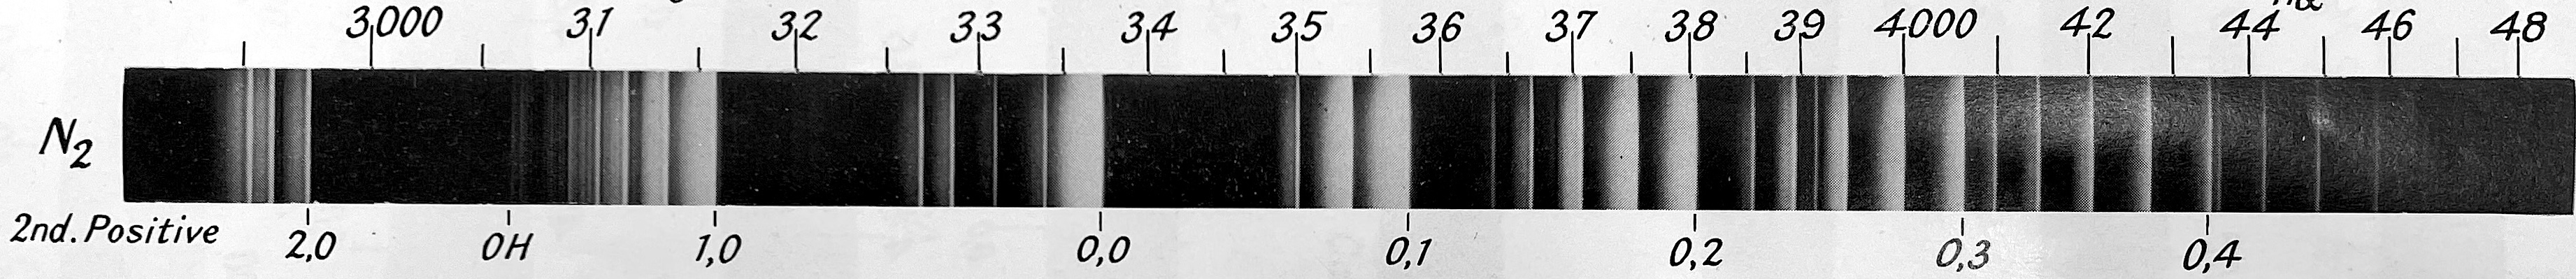
\includegraphics[width=1\textwidth]{images/N2_2PS.jpeg}
    \caption[Dinitrogen Second Positive System from literature]{Plate of the Dinitrogen Second Positive System from \cite{book}. The wavelengths are displayed above the photograph in Å.}
    \label{fig:n2_2ps}
\end{figure}


Using data from \cite{coefficients} listed in Table \ref{tab:boltzmann} (Appendix) and the OES spectrum of the plasma a Boltzmann plot is created. It is shown in Figure \ref{fig:boltzmann}. By calculating the slope of the plot from relative intensities the electron temperature can be estimated. As mentioned in \ref{sec:boltzmann} this can not be used as an absolute measurement in this work, because the plasma is non-thermal and is not in a local thermal equilibrium. From the slope obtained by fitting the data a temperature value of around 6500 K is found which appears to be in the expected order of magnitude. It lies between the values (3365 K -- 9168 K) that were found in \cite{oes_temperature} for an Argon plasma with a similar setup. This result also supports the correct identification of the observed emission peaks as transitions of the 2PS of molecular nitrogen.

\begin{figure}
    \centering
    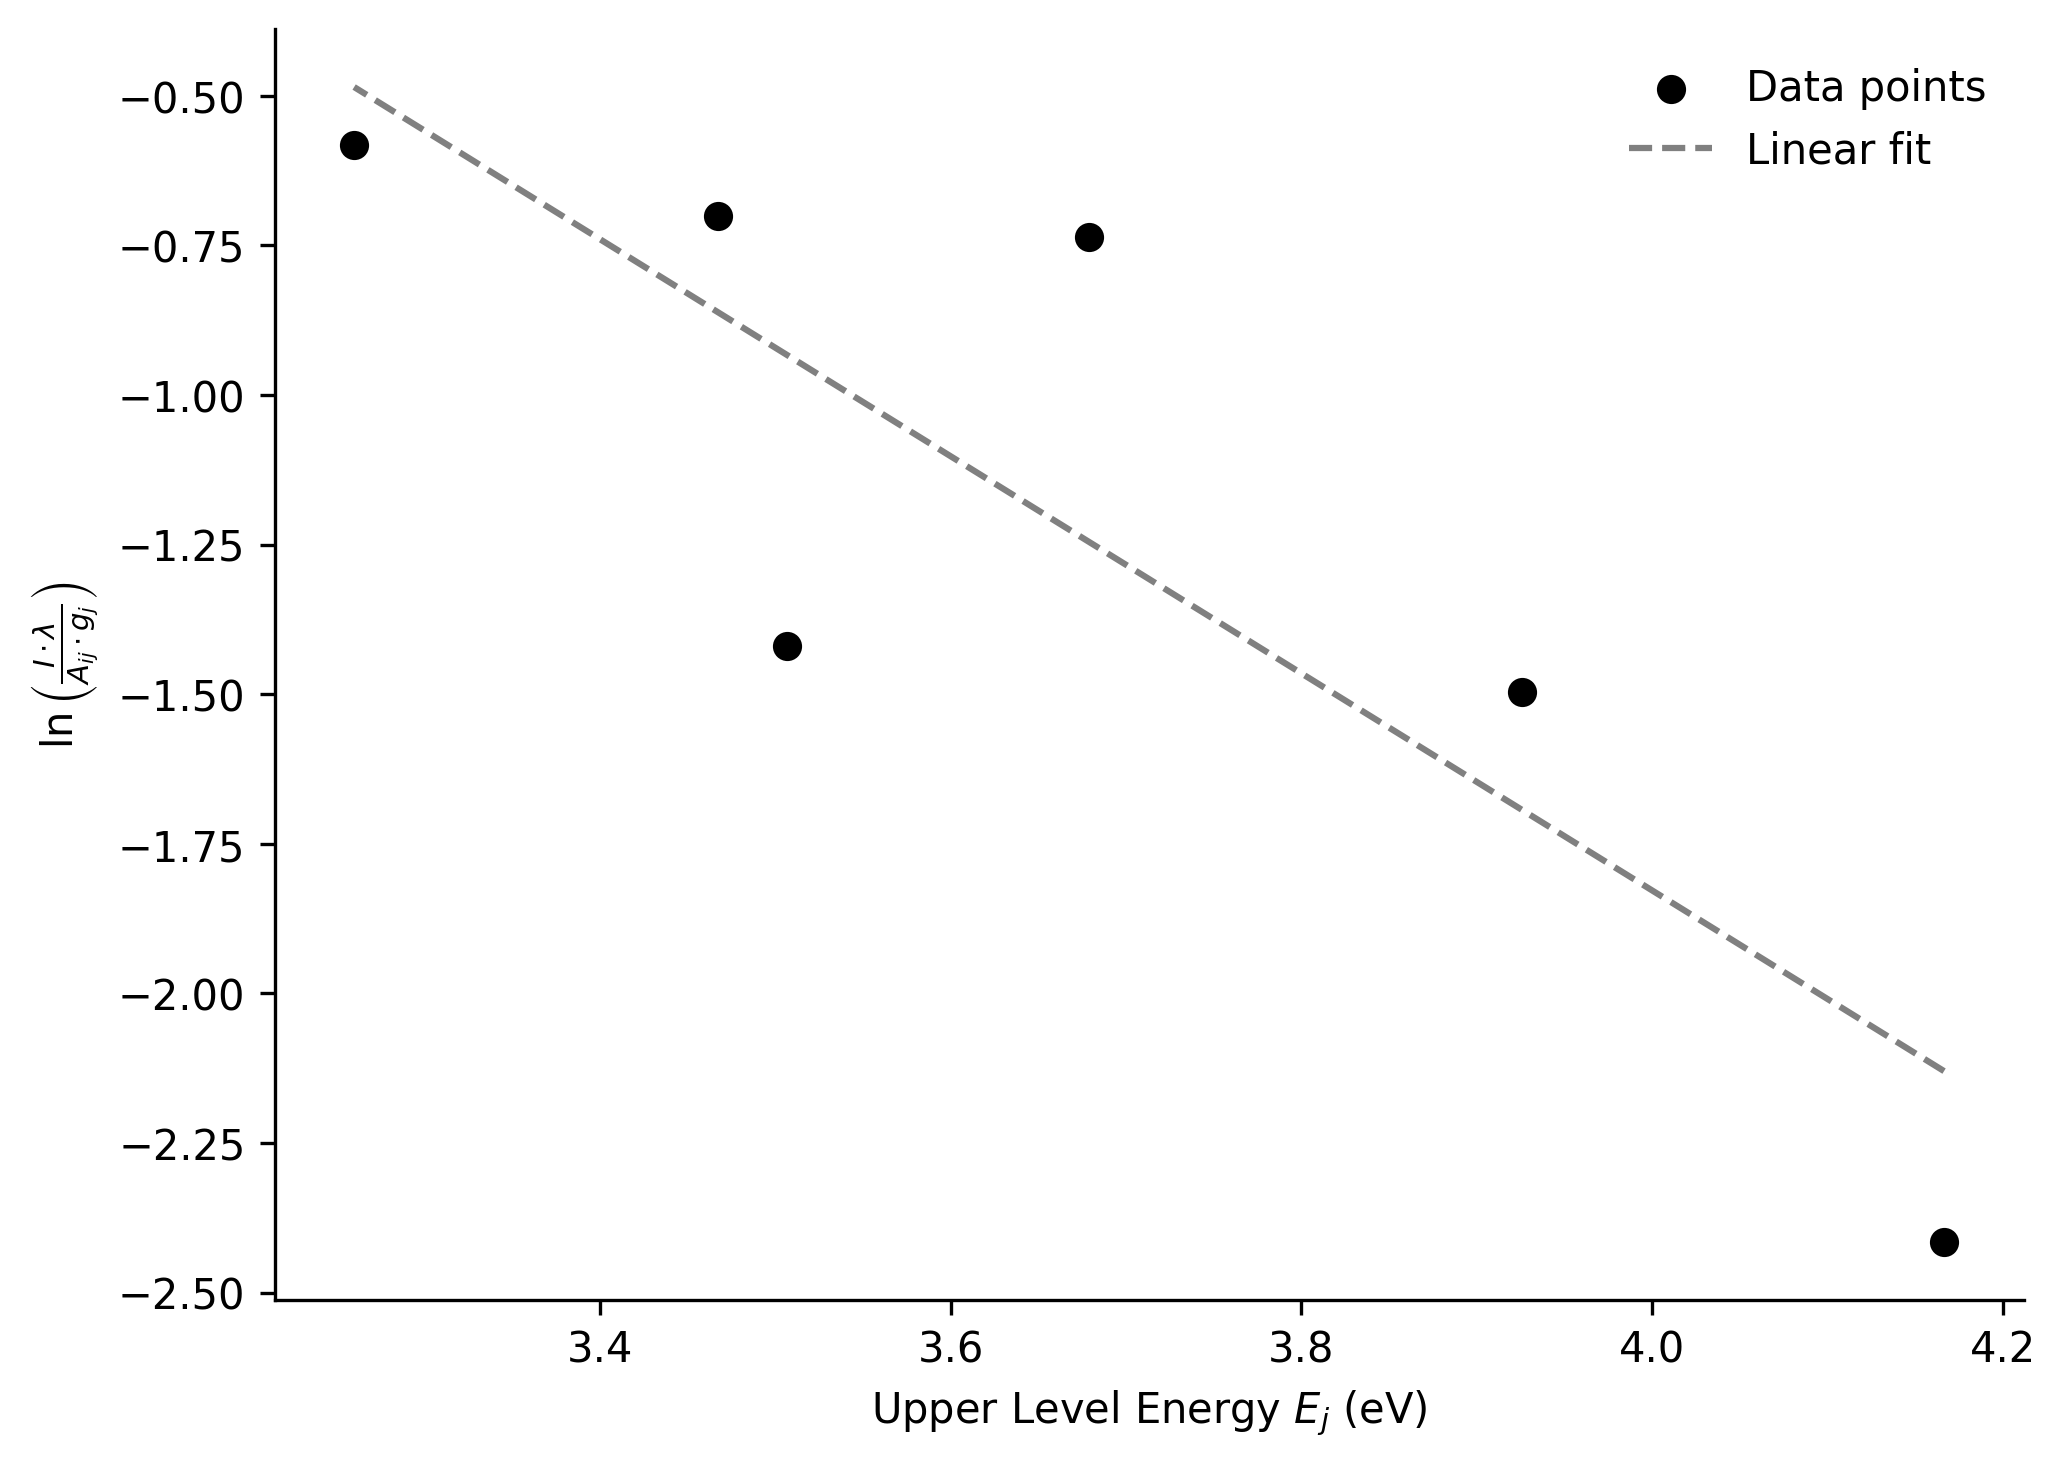
\includegraphics[width=.85\textwidth]{images/boltzmann_plot.png}
    \caption[Boltzmann Plot to estimate electron temperature]{Boltzmann Plot to estimate electron temperature using data from \cite{coefficients} listed in Table \ref{tab:boltzmann}.}
    \label{fig:boltzmann}
\end{figure}

\section{Effect of UV Exposure}
To confirm the effect of UV radiation on the spores of C. sphaerospermum, a control experiment is performed. First the spores are exposed to the UV lamp on agar medium for different times. After 15 min of exposure full deactivation was achieved. To control for the effect of the UV light on the agar medium, a second experiment is performed where the agar medium and spores are exposed to the UV light separately. To expose the spores they are instead put into the UV light in water and added to untreated agar media later. In Figure \ref{fig:uv_experiment} the petri dishes after incubation are shown. Table \ref{tab:uv_matrix} shows the number of colonies in a matrix. It becomes clear from this data that the UV light has no significant effect on the agar medium while it has a strong effect on the spores after an exposure time of 15 minutes. Using equation \ref{eq:uv_dose} the dose of UV radiation can be estimated and equates to 1.03 mJ/cm$^2$.

\begin{figure}
    \centering
    \begin{subfigure}[b]{0.6\textwidth}
        \centering
        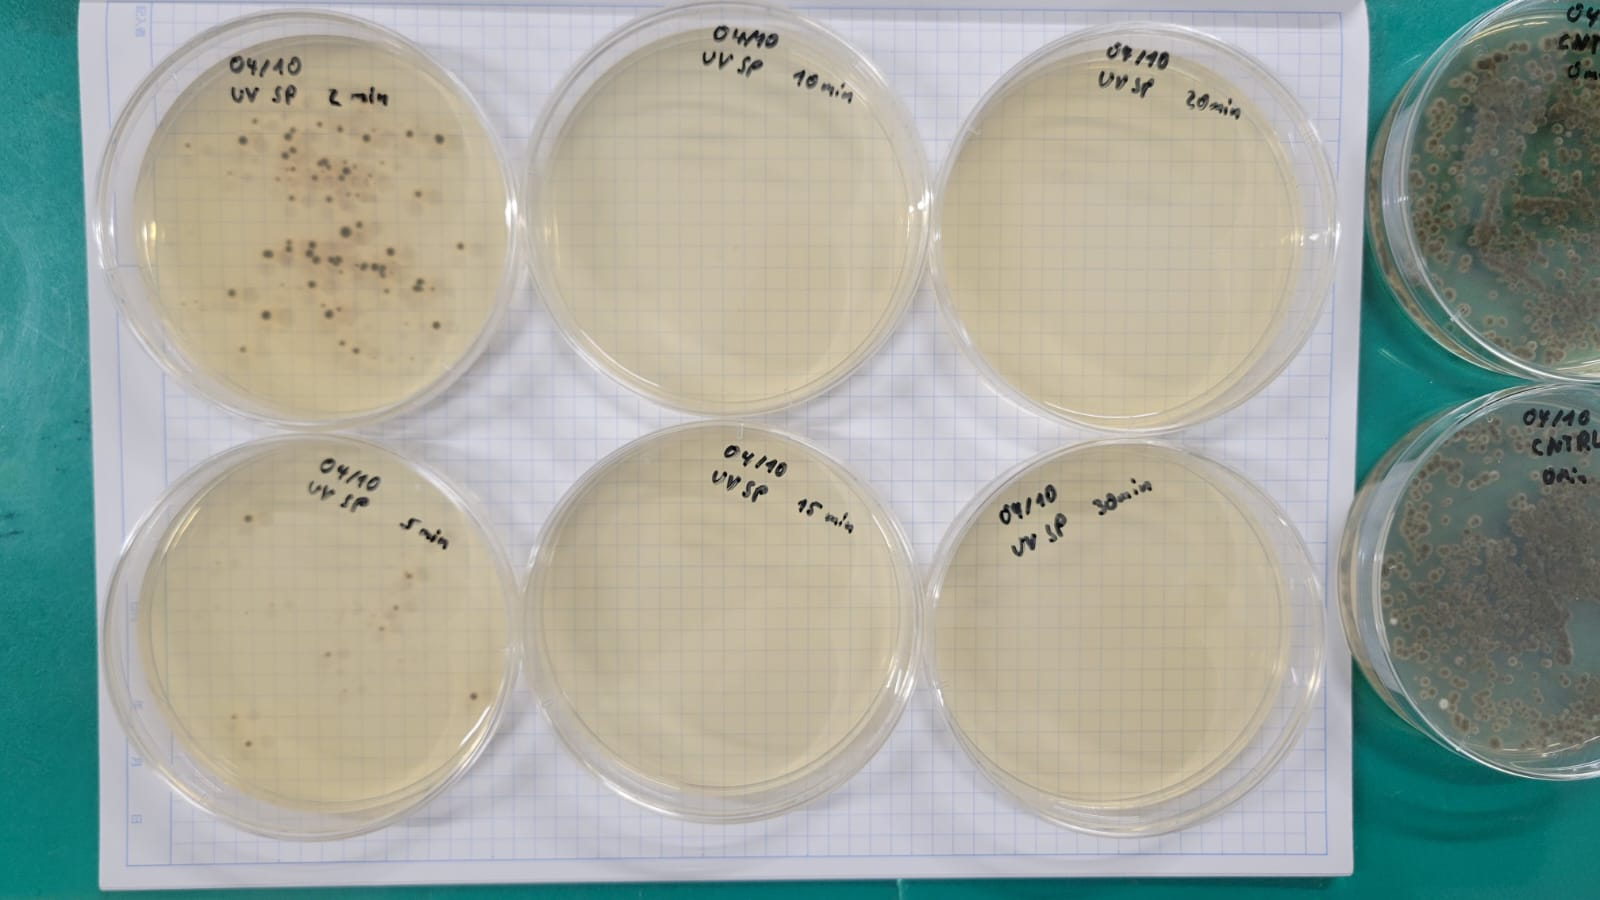
\includegraphics[width=\textwidth]{images/UV_SP.jpeg}
        \caption{Spore UV exposure}
        \label{fig:uv_a}
    \end{subfigure}
    \vfill
    \begin{subfigure}[b]{0.6\textwidth}
        \centering
        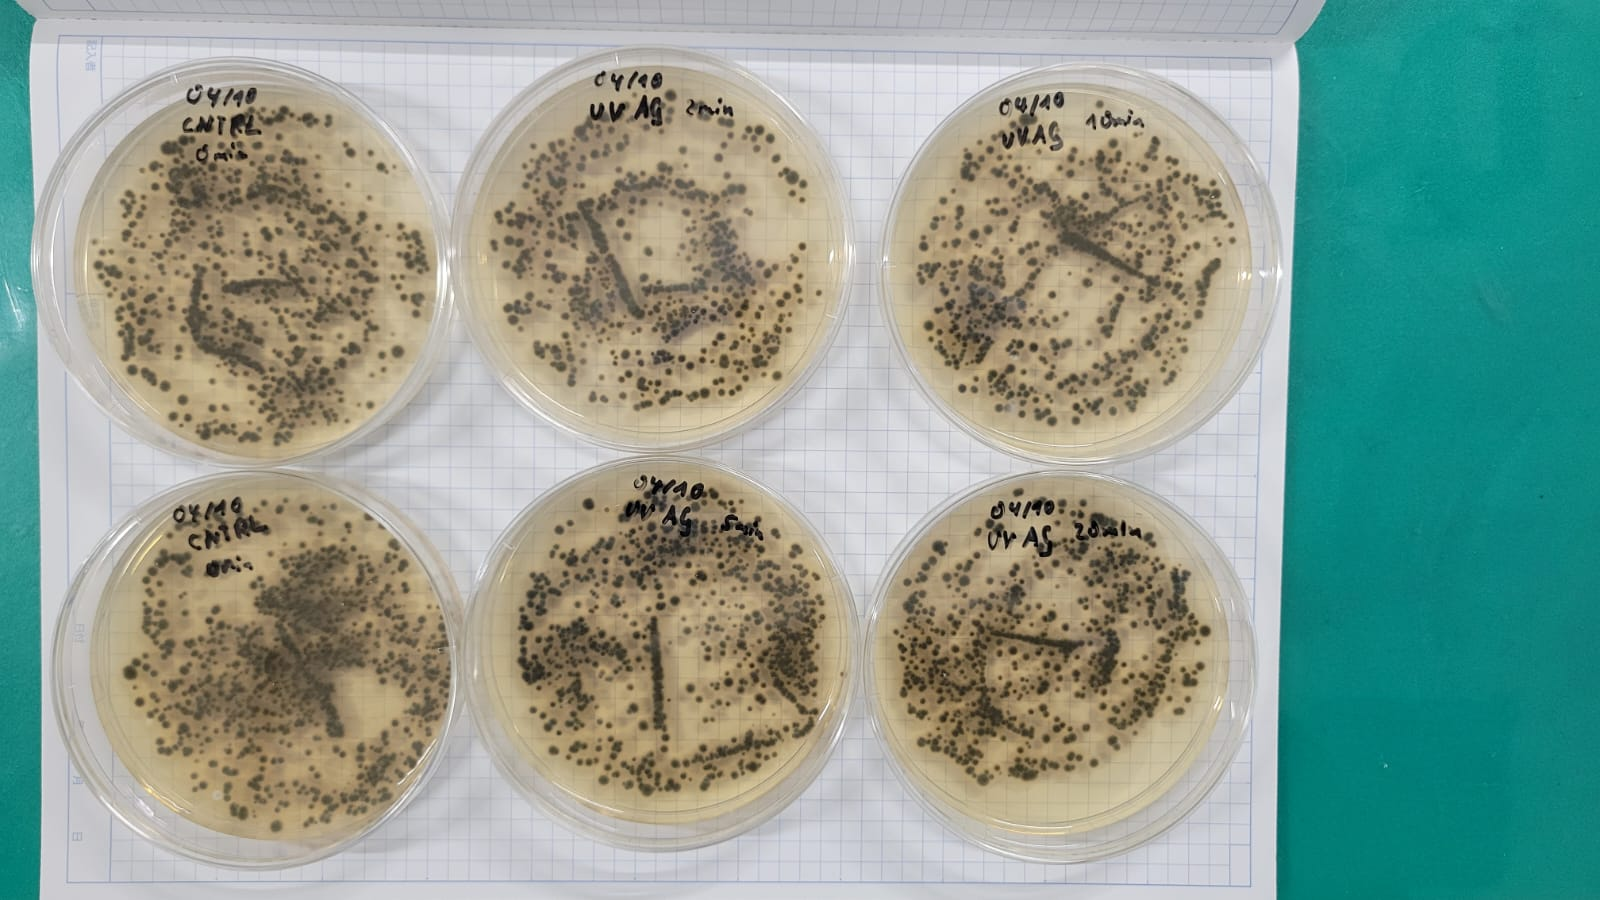
\includegraphics[width=\textwidth]{images/UV_AG.jpeg}
        \caption{Agar UV exposure}
        \label{fig:uv_b}
    \end{subfigure}
    \caption[Photograph of Petri dishes after treatment]{Petri dishes with spores (a) and agar (b) treated with UV light}
    \label{fig:uv_experiment}
\end{figure}

\begin{table}
    \centering
    \caption[Number of colonies after UV exposure as a matrix]{Number of colonies after UV exposure as a matrix. The results after 15 minutes are shown with an estimated dose of ca. 1.03 mJ/cm$^2$.}
    \vspace*{1em}
    \renewcommand{\arraystretch}{1.4}
    \setlength{\tabcolsep}{12pt}
    \begin{tabular}{c|cc}
        {\# of colonies} & {Spores no UV} & {Spores UV} \\
        \hline
        Agar no UV & >100 (cntrl) & 0 \\
        Agar UV    & >100 & 0 \\
    \end{tabular}
    \label{tab:uv_matrix}
\end{table}


\section{Effect of Plasma Treatment}
\chapter{Conclusion}
\label{chap:conclusion}
This work aimed to isolate the sterilizing effects of radiation in APP treatment on C. sphaerospermum. To summarize, this chapter will provide an overview and an assessment of the results that were found. It will also discuss the limitations of the current work and suggest possible outlooks for future work.

The results of the experiments show that the subject of this study is a relevant topic when trying to understand the effects of APP sterilization further and the research question posed were answered. While not perfectly aligning the wavelengths, the two experiments leading up to the full treatment still provided a good basis to support the results of the final experiment. It was very clearly confirmed that radiation in the UV range around 250 nm is capable of sterilizing the spores of C. sphaerospermum and the control experiment concluded that its effects on the agar media are negligible at the doses used. It was found that an estimated dose of 0.35 mJ/cm² is sufficient to sterilize the spores of C. sphaerospermum in this setting. The plasma used in the experiment was found to emit UV radiation mainly in the range of 300 nm to 400 nm. The main species that was found in the OES measurements was Nitrogen and the radiation was primarily attributed to its 2PS. While not very conclusive, a Boltzmann plot was used and found the electron temperature to be around 6500 K or roughly 0.5 eV.

The use of the UV transparent quartz glass enabled a simple experiment, which was able to show that the radiation emitted by the APP alone is capable of sterilizing the spores and might play an important role. While the data is very limited and the number of results are not statistically conclusive, the concept has been proven and a deactivation of approximately 50 \% of spores was achieved after 30 minutes. The inclusion of a control experiment that estimates the hydroxyl radical concentration provided support for the assumption that the radiation is the main contributor to the sterilization in the experiment. Gaining a better understanding for the mechanisms, like radiation, that cause APP to be effective at sterilization is crucial for the development and improvement of APP as a sterilization method. It shows potential for treatment of surfaces without touching them directly, which could be a great advantage in.

To improve the results, the concentration of hydroxyl radicals should be lowered to a level that is comparable to that of the control group. This would allow for a more direct comparison of the two experiments and would help to quantify the role of the radiation in the sterilization process. For that a better seal of the quartz glass is needed to prevent the escape of hydroxyl radicals. Also, the possibility of hydroxyl radicals being formed behind the quartz glass by the UV radiation should be considered and investigated. For that a UV blocking layer could be applied to the quartz glass so that the only source of hydroxyl radicals is the APP itself. To further categorize the plasma additional experiments should be conducted and an absolute quantification of the radiation should be performed. As discussed in section \ref{sec:oes_temperature} Akatsuka and others \cite{oes_temperature} have presented a non-intrusive method that could be used to measure the electron temperature and density of the plasma accurately. Additionally, an experiment with a UV lamp capable of emitting the same wavelengths as the APP could be performed to establish a more direct comparison.

Because of the limited time that the author spent at KIT, it was not possible to conduct any more of the proposed experiments. However, the results of the current work seem promising and may lead to further research in this area in KIT's lab.


\cleardoublepage
\renewcommand\bibname{References}
\phantomsection
\addcontentsline{toc}{chapter}{References}
\printbibliography
\cleardoublepage

\appendix
\chapter{Appendix}
\begin{table}[h]
    \centering
    \caption[$A_{ij}$ and $E_j$ values for selected N$_2$ 2PS transitions]{Spectroscopic data for selected N$_2$ Second Positive System transitions. $A_{ij}$ and $E_j$ values from Gilmore and others (1992) \cite{coefficients}.}
    \vspace*{1em}
    \begin{tabular}{llllll}
    {Wavelength in nm} & {Intensity in a.u.} & $A_{ij}$ in {$s^{-1}$} & $g_j$ & $E_j$ in {cm$^{-1}$} \\
    \hline
    297 & 1185.53  & $3.94 \times 10^6$ & 1 & 33606 \\
    315 & 8464.27  & $1.19 \times 10^7$ & 1 & 31665 \\
    337 & 18781.21 & $1.32 \times 10^7$ & 1 & 29671 \\
    353 & 3834.82  & $5.60 \times 10^6$ & 1 & 28284 \\
    357 & 12313.39 & $8.86 \times 10^6$ & 1 & 27966 \\
    380 & 5188.45  & $3.53 \times 10^6$ & 1 & 26290 \\

    \end{tabular}
    \label{tab:boltzmann}
\end{table}
\fontsize{12pt}{12pt}\selectfont
\clearpage
\end{document}